%=====================================================================
%  ISO8007 MSc Business Analytics Dissertation - Draft Version 3.0
%  Kartikey Sharma | 250559280 | Newcastle University Business School
%
%  v3 changes from v2:
%   * Restructured into the traditional Newcastle dissertation format
%     (roman front matter, Chapters 1-6, section numbering "1.1)"),
%     following the exemplar dissertation supplied by the student.
%   * In-text citations converted from superscript numerals to Harvard
%     author-date, as ISO8007 s.3.5 makes Harvard mandatory and
%     expressly forbids numbered in-text references.
%   * Prose rewritten in Indian Academic English. No em dashes used.
%   * Sections for which data are not yet available are left blank and
%     marked in a boxed notice.
%=====================================================================
\documentclass[12pt,a4paper]{article}
\usepackage[T1]{fontenc}
\usepackage[utf8]{inputenc}
\usepackage{mathptmx}
\usepackage[left=3.2cm,right=2.5cm,top=2.5cm,bottom=2.5cm]{geometry}
\usepackage{microtype}
\usepackage{booktabs}
\usepackage{longtable}
\usepackage{array}
\usepackage{tabularx}
\usepackage{ragged2e}
\usepackage{graphicx}
\usepackage{tikz}
\usetikzlibrary{arrows.meta,positioning,calc,fit,backgrounds}
\usepackage{caption}
\usepackage{enumitem}
\usepackage{setspace}
\usepackage{float}
\usepackage{titlesec}
\usepackage{titletoc}
\usepackage{amssymb}
\usepackage{amsmath}
\usepackage{etoolbox}
\usepackage[hidelinks]{hyperref}

% Ragged-right inside tables: avoids the heavy hyphenation that
% justification forces in narrow columns.
\AtBeginEnvironment{tabularx}{\RaggedRight}
\AtBeginEnvironment{longtable}{\RaggedRight}

%---------------------------------------------------------------------
%  Chapter machinery (article class, dissertation appearance)
%---------------------------------------------------------------------
\newcounter{chapno}
\setcounter{chapno}{0}
\renewcommand{\thesection}{\arabic{chapno}.\arabic{section}}
\renewcommand{\thesubsection}{\arabic{chapno}.\arabic{section}.\arabic{subsection}}
\renewcommand{\thefigure}{\arabic{chapno}.\arabic{figure}}
\renewcommand{\thetable}{\arabic{chapno}.\arabic{table}}

\titleformat{\section}{\normalsize\bfseries}{\thesection)}{1.2em}{}
\titleformat{\subsection}{\normalsize\bfseries}{\makebox[1.2em][l]{-}\thesubsection)}{0.8em}{}
\titlespacing*{\section}{0pt}{14pt}{5pt}
\titlespacing*{\subsection}{0pt}{11pt}{4pt}

\newcommand{\chapt}[2]{%
  \newpage
  \setcounter{chapno}{#1}%
  \setcounter{section}{0}\setcounter{subsection}{0}%
  \setcounter{figure}{0}\setcounter{table}{0}%
  \addtocontents{toc}{\protect\vspace{9pt}}%
  \addtocontents{toc}{\protect\noindent{\protect\bfseries Chapter #1:} #2\protect\par\protect\vspace{3pt}}%
  \begin{center}
    {\large\bfseries Chapter #1}\\[8pt]
    {\large #2}
  \end{center}
  \vspace{14pt}%
}

%---------------------------------------------------------------------
%  Captions: figure caption below and centred; table caption above
%---------------------------------------------------------------------
\captionsetup[figure]{font=small,labelfont=bf,labelsep=colon,
  justification=centering,singlelinecheck=true,skip=6pt}
\captionsetup[table]{font=small,labelfont=bf,labelsep=colon,
  justification=raggedright,singlelinecheck=false,skip=4pt}

\setlength{\parindent}{0pt}
\setlength{\parskip}{9pt}
\onehalfspacing
\renewcommand{\arraystretch}{1.15}
\newcolumntype{L}[1]{>{\RaggedRight\arraybackslash}p{#1}}

%---------------------------------------------------------------------
%  Boxes
%---------------------------------------------------------------------
\newcommand{\blankbox}[2]{%
\begin{center}
\begin{tikzpicture}
\node[draw=black,dashed,line width=0.8pt,inner sep=10pt,
 text width=0.90\textwidth]{\setstretch{1.15}\small\textbf{[THIS SECTION IS LEFT BLANK: #1]}\\[5pt]\small #2};
\end{tikzpicture}
\end{center}}

\newcommand{\nbox}[2]{%
\begin{center}
\begin{tikzpicture}
\node[draw=black,line width=0.8pt,inner sep=10pt,
 text width=0.90\textwidth]{\setstretch{1.15}\small\textbf{#1}\\[5pt]\small #2};
\end{tikzpicture}
\end{center}}

%---------------------------------------------------------------------
%  Contents list appearance: dotted leaders throughout, tight spacing
%---------------------------------------------------------------------
\makeatletter
\renewcommand*\l@section{\@dottedtocline{1}{1.2em}{3.2em}}
\renewcommand*\l@subsection{\@dottedtocline{2}{4.6em}{3.8em}}
\renewcommand*\l@figure{\@dottedtocline{1}{0em}{3.4em}}
\renewcommand*\l@table{\@dottedtocline{1}{0em}{3.2em}}
\makeatother

\begin{document}
\pagenumbering{Roman}

%=====================================================================
%  TITLE PAGE (page i)
%=====================================================================
\thispagestyle{plain}
\begin{center}
\vspace*{18pt}

{\large\bfseries NEWCASTLE UNIVERSITY BUSINESS SCHOOL}

\vspace{50pt}

{\LARGE\bfseries When Do Dashboards Override Judgement?}

\vspace{14pt}

{\large Decision Scenarios, Data Quality and Managerial Reliance\\[6pt]
on Business Intelligence Dashboards}

\vspace{60pt}

{\large\bfseries Kartikey Sharma}

\vspace{8pt}

{\large Student Number: 250559280}

\vspace{50pt}

{\large Supervisor: Dr Xinyue Hao}

\vspace{50pt}

{\large A dissertation submitted in part fulfilment of the\\[6pt]
requirements for the degree of}

\vspace{10pt}

{\large\bfseries MSc Business Analytics}

\vspace{40pt}

{\large Module ISO8007\\[6pt]
Academic Year 2025/26}

\vspace{30pt}

{\large\bfseries Draft Version 3.0}

\vspace{6pt}

{\large 25 August 2026}

\vspace{20pt}

{\small Word count of the main text: see the note on page vii.}

\end{center}

%=====================================================================
%  ACKNOWLEDGEMENTS
%=====================================================================
\newpage
\begin{center}{\large\bfseries Acknowledgements}\end{center}
\vspace{12pt}

At the outset, I wish to record my sincere gratitude to my supervisor, Dr Xinyue Hao, for her guidance
throughout this study, and in particular for her insistence that the research questions be framed
conditionally rather than assuming at the outset the very behaviour that this study sets out to examine.
That single correction has shaped the entire design.

I am also grateful to the examiners of the NBS8062 research proposal. Their observations regarding the
coherence of the conceptual argument and the specificity of the secondary data strand were exacting, and
they have improved this work in a direct and material manner.

I would further like to thank Nick Howey, Dissertation Co-ordinator for the MSc Business Analytics
programme, for administrative guidance during the course of the module, and the staff of the Philip
Robinson Library for assistance in accessing several of the primary regulatory documents upon which
Chapter 4 depends.

Finally, I wish to thank my family for their unfailing support during my period of study in the United
Kingdom. Any errors that remain in this work are entirely my own.

%=====================================================================
%  ABSTRACT
%=====================================================================
\newpage
\begin{center}
{\large\bfseries When Do Dashboards Override Judgement?}\\[6pt]
{\large Decision Scenarios, Data Quality and Managerial Reliance on\\[4pt]
Business Intelligence Dashboards}
\end{center}
\vspace{12pt}

{\setstretch{1.24}
Business intelligence dashboards have become the point at which the majority of managerial decisions now
begin. A substantial body of literature establishes that managers do rely upon such systems. Comparatively
little, however, is known regarding the conditions under which that reliance ceases to assist judgement and
begins to displace it. This study accordingly asks not whether managers defer to dashboards, but rather in
which decision scenarios they do so, for what reasons, and with what consequence for decision accuracy and
for the generation of alternative courses of action. An integrated behavioural framework is developed which
links dashboard design and visual framing, the visibility of data quality defects, and the organisational
accountability regime to three decision outcomes. A pragmatic orientation resting upon a critical realist
ontology is adopted, and the design is mixed method across three strands, namely a scenario based decision
experiment employing experimental vignette methodology, a structured documentary analysis of publicly
evidenced analytics failures, and semi structured interviews sampled upon observed experimental behaviour.
The documentary strand has been completed and is reported in full. Twelve organisational failures were
coded against a fixed extraction frame, drawing exclusively upon regulator enforcement notices, statutory
inquiry reports and royal commission findings across nine sectors and four jurisdictions. Two patterns
emerge from the coding. Firstly, defects which were silent at the point of use persisted for a period of
years, whereas defects producing any perceptible signal were recognised within hours or days. Secondly, and
of greater consequence, in nine of the twelve cases a human challenge to the system output was in fact
raised and was thereafter overridden, ignored or not acted upon. This second finding obliges a revision of
the framework with which the study commenced. Attentional accounts of automation bias explain why a manager
might fail to notice a defect, but they do not explain why noticing repeatedly failed to produce action.
The study therefore distinguishes detection failure from authority failure, and proposes legitimacy
asymmetry as the mechanism which connects the two. The practical implication is that governance investment
directed towards better warnings addresses the wrong constraint. The experimental and interview strands
remain in the field at the date of this draft, and the sections which depend upon them have been left blank
and marked accordingly.
\par}

\vspace{10pt}
{\bfseries Keywords:} business intelligence dashboards; managerial judgement; over-reliance; data quality;
mixed methods.

%=====================================================================
%  CONTENTS
%=====================================================================
\newpage
\begin{center}{\large\bfseries Contents}\end{center}
\vspace{6pt}
\makeatletter
{\setstretch{1.1}\setlength{\parskip}{0pt}
\renewcommand{\@dotsep}{2.5}
\setcounter{tocdepth}{2}
\@starttoc{toc}
\par}

%=====================================================================
%  LIST OF FIGURES
%=====================================================================
\newpage
\begin{center}{\large\bfseries List of Figures}\end{center}
\vspace{6pt}
{\setstretch{1.1}\setlength{\parskip}{0pt}\@starttoc{lof}\par}

%=====================================================================
%  LIST OF TABLES
%=====================================================================
\newpage
\begin{center}{\large\bfseries List of Tables}\end{center}
\vspace{6pt}
{\setstretch{1.1}\setlength{\parskip}{0pt}\@starttoc{lot}\par}
\makeatother

%=====================================================================
%  ABBREVIATIONS AND NOTES
%=====================================================================
\newpage
\begin{center}{\large\bfseries Abbreviations}\end{center}
\vspace{10pt}

{\setstretch{1.2}
\begin{tabular}{@{}p{2.6cm} p{11.5cm}@{}}
BI & Business intelligence \\
CAA & Civil Aviation Authority (United Kingdom) \\
CI & Confidence interval \\
FCA & Financial Conduct Authority (United Kingdom) \\
GDPR & General Data Protection Regulation \\
KPI & Key performance indicator \\
MRS & Market Research Society \\
NATS & National Air Traffic Services (United Kingdom) \\
OCC & Office of the Comptroller of the Currency (United States) \\
OSR & Office for Statistics Regulation (United Kingdom) \\
PHE & Public Health England \\
RQ & Research question \\
SEC & Securities and Exchange Commission (United States) \\
TSB & TSB Bank plc \\
\end{tabular}
\par}

\vspace{22pt}
\begin{center}{\large\bfseries Note on the Status of this Draft}\end{center}
\vspace{10pt}

This is Draft Version 3.0 and it is not the final submission. Chapters 1, 2 and 3 are complete. Chapter 4
reports the documentary strand, which has been completed in full. The scenario based decision experiment
and the semi structured interviews remain in the field at the date of this draft. Every section of the
document which depends upon those two strands has been left blank and is marked by a boxed notice stating
what will be reported in that place and what data are awaited. No result has been estimated, simulated or
otherwise supplied in place of data not yet collected. Chapters 5 and 6 are consequently provisional and
will be rewritten once all three strands have reported.

\vspace{10pt}
\begin{center}{\large\bfseries Statement on the Use of Generative Artificial Intelligence}\end{center}
\vspace{10pt}

Generative artificial intelligence tools have been used to assist with document formatting, the preparation
of figures from coded data, and language editing. All research design decisions, source selection, coding
judgements, analysis and interpretation are my own. Every source cited has been checked against its primary
record and is listed with its access route in the accompanying reference register, which is described at
Appendix~D.

\vspace{10pt}
\begin{center}{\large\bfseries Word Count}\end{center}
\vspace{10pt}

Main text of Chapters 1 to 6, inclusive of tables and figure captions: approximately \textbf{11,580}
words, against the limit of 12,000 words specified at section 2.4 of the ISO8007 guidelines. The title
page, contents, acknowledgements, abstract, abbreviations, references and appendices are excluded from this
count, in accordance with those guidelines. It should be noted that sections 4.3, 4.4, 4.5 and part of
section 5.4 are presently blank. When those sections are written, a corresponding reduction will be
required elsewhere in the main text in order to remain within the limit.

\newpage
\pagenumbering{arabic}
\setcounter{page}{1}

%=====================================================================
\chapt{1}{Introduction}
%=====================================================================

\section{Background}

Managerial decision making in the contemporary organisation rarely commences with a blank sheet of paper.
It commences with a screen. Over the past two decades, business intelligence dashboards have evolved from
comparatively passive reporting interfaces into what may reasonably be termed decision infrastructure. They
determine which indicators are placed before the manager, which are aggregated away, which are shaded red,
and, most consequentially of all, which account of organisational reality proves easiest to defend at the
time when the decision is subsequently questioned.

The literature has by and large been favourable towards these systems, and not without reason.
Business intelligence capabilities are consistently associated with improved decision support and
improved organisational performance, principally because such systems integrate dispersed data,
visualise performance and embed analysis within routine managerial work (Chen, Chiang and Storey,
2012; Elbashir, Collier and Davern, 2008; Seddon et al., 2017; Trieu, 2017). In operations and
supply chain settings in particular,
dashboards support demand monitoring, inventory visibility and disruption response (Gunasekaran et
al., 2017; Kache and Seuring, 2017). The benefit is real and the present study does not seek to
dispute it.

What is less well understood is the other side of the ledger. A dashboard does not display reality. It
composes reality. In selecting indicators, aggregating complexity, assigning colours and ranking
priorities, the interface necessarily renders certain forms of knowledge more visible than others (Pauwels
et al., 2009; Sarikaya et al., 2019; Yigitbasioglu and Velcu, 2012). This compression is simultaneously the
source of the value of the dashboard and the source of its risk. A dashboard may therefore become a quiet
governor of judgement, polished, auditable and persuasive, even in circumstances where the underlying data
happen to be incomplete, delayed or excessively aggregated.

\section{The research problem}

The stakes involved are not hypothetical, and it is worthwhile grounding the problem in the public record
before proceeding to theory. The Post Office Horizon IT Inquiry found that system generated accounting data
was treated as authoritative over the contrary accounts of several hundred sub-postmasters, with
consequences that were by any measure catastrophic (Post Office Horizon IT Inquiry, 2025). The Royal
Commission into the Robodebt Scheme in Australia documented the manner in which a debt raising system built
upon averaged income data reversed the onus of proof onto citizens, and the manner in which internal legal
advice questioning its lawfulness was obtained and thereafter set aside (Royal Commission into the Robodebt
Scheme, 2023). In an entirely different setting, the independent review commissioned by the United Kingdom
Civil Aviation Authority into the flight planning failure of 2023 at NATS described how the response of an
automated system to a single ambiguous input propagated into national disruption, and how escalation to the
engineers capable of diagnosing the fault proved slower than the failure itself (Civil Aviation Authority,
2024).

On a close reading, these are not stories concerning badly designed software. They are stories concerning
what happens when a system output becomes more institutionally credible than a human objection. That
distinction is the point of departure for the present study.

The difficulty is that the literature has largely established \emph{that} reliance upon analytical outputs
occurs, without specifying with any precision \emph{under which decision conditions} such reliance becomes
hazardous, and \emph{why} organisational context makes it rational for the individual manager to defer even
in circumstances where deference proves costly for the organisation. Indeed, the evidence on the point is
genuinely contested. Individuals may be markedly averse to algorithmic advice after having observed it to
err (Dietvorst, Simmons and Massey, 2015), and yet under other conditions they display a clear preference
for algorithmic over human judgement (Logg, Minson and Moore, 2019). Systematic reviews conclude that
reliance is best understood as being condition dependent rather than as a stable individual trait (Burton,
Stein and Jensen, 2020; Mahmud et al., 2022). If that conclusion is sound, then the useful research
question must itself be conditional in its framing.

\section{Research aim and objectives}

The aim of this study is to identify the decision conditions under which managers prioritise business
intelligence dashboard outputs over intuition and contextual judgement, to explain why such prioritisation
occurs and becomes entrenched, and to assess the consequences thereof for decision accuracy and for the
generation of alternative courses of action.

The objectives of the study are as under.

\begin{enumerate}[leftmargin=*,itemsep=2pt,topsep=4pt]
\item To establish experimentally how decision risk, the visibility of data quality signals and
accountability framing jointly affect the probability that a manager follows a dashboard output which
conflicts with contextual evidence.
\item To measure whether dashboard deference is associated with a reduced generation of alternative courses
of action.
\item To characterise, from publicly evidenced organisational failures, the manner in which analytics and
reporting errors persist undetected, and whether human challenge was raised, escalated or overridden.
\item To explain, through the accounts of practising professionals, why dashboard outputs acquire greater
institutional legitimacy than contextual judgement.
\item To develop a governance framework for preserving analytical rigour whilst at the same time protecting
human challenge.
\end{enumerate}

\section{Research questions}

Two research questions are posed, each with two sub-questions. The conditional framing of the first
question is deliberate and follows directly from the contested state of the evidence noted at section 1.2
above.

\nbox{Research questions}{%
\textbf{RQ1 (when, and with what consequence).} In what decision scenarios do managers prioritise business
intelligence dashboard outputs over intuition and contextual judgement, and how does that prioritisation
relate to decision accuracy and to the generation of alternative courses of action?\\[4pt]
\hspace*{12pt}\textbf{RQ1a} How do decision risk, data quality signal visibility, accountability framing and
metric salience affect the likelihood of following a dashboard output which conflicts with contextual
evidence?\\[2pt]
\hspace*{12pt}\textbf{RQ1b} Is dashboard deference associated with a narrower generation of alternative
actions, after controlling for experience and sector?\\[6pt]
\textbf{RQ2 (why).} Why do managers prioritise dashboard outputs in those scenarios, and what organisational
conditions entrench or interrupt that prioritisation?\\[4pt]
\hspace*{12pt}\textbf{RQ2a} What reasons do professionals offer, whether perceived objectivity,
auditability, time pressure or professional defensibility, for following or for challenging dashboard
outputs?\\[2pt]
\hspace*{12pt}\textbf{RQ2b} What governance, cultural or role conditions make challenge possible?}

\section{Scope and boundaries of the study}

Three boundaries require to be stated at the outset, since a study of this length cannot possibly address
everything which the topic invites.

Firstly, the unit of analysis is the individual decision episode rather than the organisation or the
system. The study does not evaluate dashboard software as such, nor does it assess the return on analytics
investment.

Secondly, the study concerns business intelligence dashboards and organisational analytics rather than
generative artificial intelligence. Recent work on reliance upon artificial intelligence is drawn upon in
those places where the underlying mechanism is shared (Buçinca, Malaya and Gajos, 2021; Vasconcelos et al.,
2023), but generative systems introduce questions of fluency and fabrication which lie outside the present
design.

Thirdly, the study is concerned with professional decision making in commercial and public sector settings
in which dashboards are used at least weekly. It makes no claim in respect of consumer or clinical
contexts, in which the automation bias literature is considerably better developed (Goddard, Roudsari and
Wyatt, 2012; Lyell and Coiera, 2017).

\section{Significance and contribution}

The intended contribution is a condition specific account of dashboard reliance. Rather than
asking whether analytics adds value, which the literature has largely answered in the affirmative,
the study asks when analytics creates fragility, and it triangulates the answer across three
distinct evidential bases, namely experimental behaviour under controlled variation, documented
organisational failure, and the explanations offered by practising professionals. The significance
of the topic for an external reader may be stated briefly. Organisations continue to invest
heavily in analytics on the assumption that better information produces better decisions. The
failures referred to at section 1.2 indicate that this assumption holds only under conditions
which are seldom specified. Establishing what those conditions are is therefore of direct
practical value to any organisation which places a dashboard in front of a decision maker.

\section{Structure of the research}

The remainder of this dissertation is organised into five further chapters, as depicted at
Figure~\ref{fig:structure}. Chapter 2 reviews the literature as a single connected argument,
appraises the evidence critically and states the research gap. Chapter 3 sets out the
philosophical position, the design alternatives considered and rejected, the three empirical
strands, the quality criteria and the ethical safeguards. Chapter 4 presents the findings,
commencing with the completed documentary strand. Chapter 5 discusses those findings against the
conceptual framework and proposes a revision to it. Chapter 6 concludes, proposes a governance
framework, and identifies limitations and directions for further research.

\begin{figure}[H]
\centering
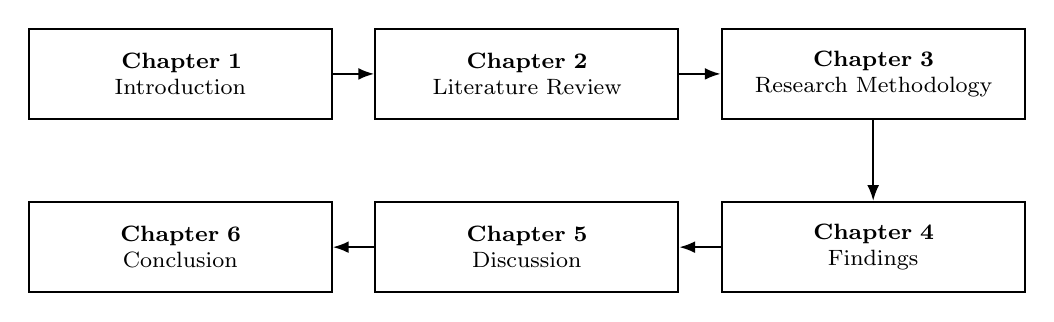
\begin{tikzpicture}[
  every node/.style={font=\footnotesize},
  ch/.style={draw=black,line width=0.7pt,align=center,inner sep=5pt,text width=3.5cm,minimum height=1.15cm},
  ar/.style={-{Latex[length=2mm]},line width=0.7pt}]
\node[ch] (c1) at (0,0) {\textbf{Chapter 1}\\Introduction};
\node[ch] (c2) at (4.4,0) {\textbf{Chapter 2}\\Literature Review};
\node[ch] (c3) at (8.8,0) {\textbf{Chapter 3}\\Research Methodology};
\node[ch] (c4) at (8.8,-2.2) {\textbf{Chapter 4}\\Findings};
\node[ch] (c5) at (4.4,-2.2) {\textbf{Chapter 5}\\Discussion};
\node[ch] (c6) at (0,-2.2) {\textbf{Chapter 6}\\Conclusion};
\draw[ar] (c1) -- (c2);
\draw[ar] (c2) -- (c3);
\draw[ar] (c3) -- (c4);
\draw[ar] (c4) -- (c5);
\draw[ar] (c5) -- (c6);
\end{tikzpicture}
\caption{Structure of the research}
\label{fig:structure}
\end{figure}

%=====================================================================
\chapt{2}{Literature Review}
%=====================================================================

\section{Scope and method of the review}

The review was conducted through structured searches of Scopus, Web of Science and Business Source
Premier, supplemented by forward and backward citation chaining from the five most central papers.
Five search strings were employed, combining terms for business intelligence dashboards,
algorithmic reliance and automation bias, data quality, creativity and option generation, and the
unintended consequences of performance management. Retrieval was restricted to peer reviewed
journal articles in the English language, with a principal window of 2015 to 2026 and no lower
bound for foundational works retained by hand. Conference proceedings were admitted only where the
venue constitutes the principal outlet for the field, which applies to human computer interaction
research. Grey literature was admitted only where it constitutes primary evidence for the
documentary strand, in which case the admissibility rules at section 3.5.2 apply. The search
documentation is placed at Appendix~G. It is pertinent to note that the review is organised as one
continuous argument rather than as a series of parallel summaries, since the contribution of the
study rests upon the connections between these literatures rather than upon any one of them taken
individually. The argument proceeds in five linked steps, as depicted at
Figure~\ref{fig:lrstructure}, and section 2.7 thereafter appraises the quality of the evidence
supporting each step.

\begin{figure}[H]
\centering
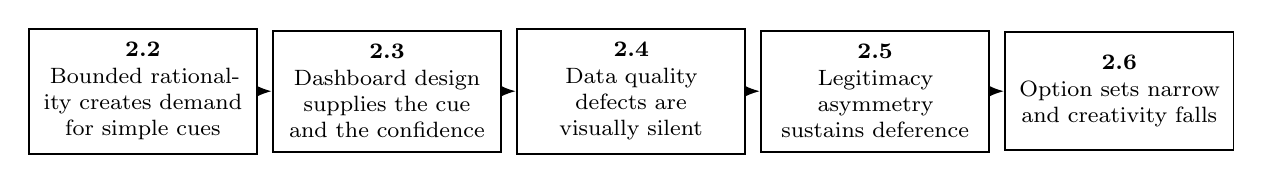
\begin{tikzpicture}[
  every node/.style={font=\footnotesize},
  st/.style={draw=black,line width=0.7pt,align=center,inner sep=5pt,text width=2.55cm,minimum height=1.5cm},
  ar/.style={-{Latex[length=2mm]},line width=0.7pt}]
\node[st] (s1) at (0,0) {\textbf{2.2}\\Bounded rationality creates demand for simple cues};
\node[st] (s2) at (3.1,0) {\textbf{2.3}\\Dashboard design supplies the cue and the confidence};
\node[st] (s3) at (6.2,0) {\textbf{2.4}\\Data quality defects are visually silent};
\node[st] (s4) at (9.3,0) {\textbf{2.5}\\Legitimacy asymmetry sustains deference};
\node[st] (s5) at (12.4,0) {\textbf{2.6}\\Option sets narrow and creativity falls};
\draw[ar] (s1) -- (s2); \draw[ar] (s2) -- (s3); \draw[ar] (s3) -- (s4); \draw[ar] (s4) -- (s5);
\end{tikzpicture}
\caption{Structure of the literature review as a single causal argument}
\label{fig:lrstructure}
\end{figure}

\section{Bounded rationality and the demand for simplified cues}

Managers satisfice. The behavioural model of rational choice advanced by Simon (1955) establishes that
decision makers operate under limits of information, time and cognitive capacity, and consequently adopt
simplifying strategies which are adequate rather than optimal. Kahneman (2011) subsequently distinguished
fast and associative processing from slow and effortful processing, and observed that expertise yields
reliable pattern recognition only in those environments which supply consistent feedback.

A dashboard is an unusually attractive satisficing device. It converts a high dimensional problem
into a small number of pre-evaluated signals at almost negligible cognitive cost. Consider a
regional operations manager who must decide on a Monday morning whether to authorise expedited
freight for a product line. The complete problem involves supplier reliability, port congestion,
contract terms, seasonality and the working capital position. The dashboard offers a single amber
indicator reading `service level at risk'. The manager is not being lazy in attending to that
indicator. She is behaving exactly as Simon (1955) would predict.

The implication is directional and requires to be stated with care. Bounded rationality does not predict
that managers will believe dashboards to be true. It predicts that under time pressure they will
\emph{cease searching} once a sufficiently authoritative looking cue becomes available. The behavioural
question is therefore not one of belief but rather one of search termination, and search termination is
precisely what dashboard design governs.

\section{From cognition to interface: design, salience and confidence}

If bounded rationality creates the demand for simplified cues, then dashboard design determines
the supply of them. Research on performance dashboards demonstrates that layout, metric selection,
update frequency and visual encoding shape both interpretation and use (Pauwels et al., 2009;
Yigitbasioglu and Velcu, 2012). Sarikaya et al. (2019) demonstrated, through an analysis of a
large corpus of real dashboards, that the term covers a wide design space whose variants afford
sharply different behaviours, ranging from open exploration to compliance oriented monitoring, and
Bach et al. (2023) have since catalogued the recurring patterns through which dashboards structure
attention. Underpinning all of this, foundational visualisation research explains the mechanism,
in that graphical perception and visual encoding determine what users notice and how accurately
they read quantitative information (Cleveland and McGill, 1984; Tufte, 2001; Ware, 2013).

The transition from cognition to interface is therefore causal rather than merely thematic. Where Simon
(1955) explains why a manager will accept a simplified cue, visualisation research explains which cue that
will be, namely the one possessing the highest visual salience, and how confident the manager will feel
whilst accepting it. Confidence is the pivotal variable in this regard. A red, amber and green indicator
does not merely summarise a position. It signals that the interpretive work has already been completed by
somebody else.

The behavioural consequence is well documented in the automation bias literature. Individuals misuse
automation by accepting system outputs too readily (Parasuraman and Riley, 1997), and automated cues
encourage acceptance even in circumstances where contradictory evidence is available (Mosier et al., 1998;
Skitka, Mosier and Burdick, 1999). Parasuraman and Manzey (2010) integrated these findings through
attention, arguing that reliance reduces the attentional sampling of raw evidence. Systematic reviews
conducted in clinical settings confirm both the frequency of the effect and its sensitivity to verification
cost, in that the harder it is to check the system, the more readily it is trusted (Goddard, Roudsari and
Wyatt, 2012; Lyell and Coiera, 2017).

The contemporary literature nonetheless rejects any simple account in which people merely
over-trust machines. Observing an algorithm to err produces disproportionate abandonment of it
(Dietvorst, Simmons and Massey, 2015), whilst other tasks reveal a general preference for
algorithmic over human judgement (Logg, Minson and Moore, 2019). The apparent contradiction is
resolved by reviews which conclude that reliance varies with task type, perceived expertise, error
visibility and retained control (Burton, Stein and Jensen, 2020; Mahmud et al., 2022). This is the
single most important justification for the conditional framing of RQ1. Studies of artificial
intelligence assisted decision making extend the point usefully, since over-reliance may be
reduced by cognitive forcing functions which raise the cost of uncritical acceptance (Buçinca,
Malaya and Gajos, 2021), and explanations reduce over-reliance only where engaging with the
explanation is less effortful than performing the task oneself (Vasconcelos et al., 2023).
Reliance would appear, then, to be an engineering and governance variable rather than a
personality trait.

\section{Why data quality is a behavioural problem}

Data quality is conventionally defined across the dimensions of accuracy, timeliness, completeness,
consistency and relevance (Wang and Strong, 1996), and it must be assessed in context, since information
which is technically available may nonetheless be unfit for a particular decision task (Pipino, Lee and
Wang, 2002; Strong, Lee and Wang, 1997). Poor data quality imposes a substantial organisational cost
(Redman, 1998), and it remains a managerial rather than a purely technical responsibility which most
organisations systematically under-measure (Nagle, Redman and Sammon, 2020). Decision quality in big data
settings depends upon the whole decision chain rather than upon the data alone (Janssen, van der Voort and
Wahyudi, 2017), and upstream data problems compound invisibly into downstream cascades in high stakes
systems (Sambasivan et al., 2021).

The behavioural argument which is advanced here, and which is largely absent from that literature, is that
data quality defects are dangerous \emph{because they are visually silent}. An outdated metric, a partial
extract or an inconsistent definition renders on the screen exactly as cleanly as a valid one. There is no
perceptual difference whatsoever between a trustworthy green indicator and an untrustworthy one.

A concrete illustration may be of assistance. Let us suppose that a demand dashboard draws upon a
nightly extract which, owing to a change in an upstream schema, has silently ceased to ingest one
of fourteen regional feeds. The dashboard will not display an error. It will display a slightly
lower national demand figure, in the same typeface, colour and position as always, and the manager
who reviews it experiences no cue whatsoever that anything is amiss. This may be contrasted with a
dashboard displaying a small banner reading `data as at 12 August; 1 of 14 feeds not received'.
The underlying defect is identical. The behavioural situation is entirely different.

Combining this step with the preceding one produces the core prediction of the study, namely that the harm
arising from poor data quality is not proportional to the magnitude of the error but rather to the
confidence with which the error is displayed. This motivates the experimental manipulation of signal
visibility which is described at section 3.5.1. Where the defect is signalled, verification cost falls and
challenge should accordingly rise. Where the defect is hidden, the manager possesses no cue capable of
triggering the slower processing which Kahneman (2011) describes.

\section{Legitimacy asymmetry}

Individual cognition alone cannot explain persistent deference, for the straightforward reason that
experienced managers do frequently suspect that a dashboard is wrong. Something further is required, and
that something is institutional in character.

Decision support systems are not neutral tools. They participate in organisational knowing and
reshape decision routines (Arnott and Pervan, 2005; Shollo and Galliers, 2016). Performance
measurement systems generate well documented unintended consequences, amongst which are gaming,
tunnel vision and the displacement of judgement by measurable proxies (Franco-Santos and Otley,
2018). Espeland and Sauder (2007) demonstrated reactivity, in that once a measure becomes publicly
consequential, organisations reorganise around it, and the measure begins to constitute the very
reality which it claims merely to describe.

From these strands the study derives its central organisational construct, namely \emph{legitimacy
asymmetry}. The argument may be stated quite simply. A dashboard based decision is standardised, visual,
auditable and defensible after the event. A judgement based objection, by contrast, is contextual, tacit
and difficult to document. When outcomes are subsequently reviewed, the statement that `the dashboard
showed green' constitutes a complete defence, whereas the statement that `it did not feel right to me' does
not. The asymmetry is therefore not one of accuracy but rather one of \emph{defensibility}.

Supporting evidence is available from adjacent literatures. Algorithmic systems function as instruments of
organisational control rather than merely as sources of information (Kellogg, Valentine and Christin,
2020), and professionals disengage their critical judgement in circumstances where system opacity renders
challenge professionally risky (Lebovitz, Lifshitz-Assaf and Levina, 2022). The resulting design problem
may usefully be framed as one of allocating decision authority as between humans and systems (Shrestha,
Ben-Menahem and von Krogh, 2019).

Legitimacy asymmetry thus explains what cognition alone cannot, namely that deference may be individually
rational even where it is organisationally costly. It also generates a testable prediction, that framing a
decision as auditable should raise deference independently of the underlying data, which is examined as H2
below.

\section{Option-set narrowing and creative exploration}

Creativity is treated here not as an artistic quality but rather as a decision quality outcome,
namely the capacity to generate alternative interpretations and courses of action under
uncertainty. Evaluation pressure, control and rigid performance systems have been shown to reduce
creative output (Amabile, 1998). Organisational creativity resides in the interaction of
individual, group and contextual conditions (Woodman, Sawyer and Griffin, 1993), creativity is
defined through the joint criteria of originality and effectiveness (Runco and Jaeger, 2012), and
the state of the science synthesis of Anderson, Potočnik and Zhou (2014) confirms its contextual
contingency.

The specific mechanism proposed here is \emph{option-set narrowing}. A dashboard does not forbid
alternatives. It renders certain options visible and pre-quantified whilst leaving others
unmeasured and considerably harder to argue for. Under time pressure and accountability, the
unmeasured option is not so much rejected as never seriously formulated. Returning to the freight
example, expediting the shipment appears upon the dashboard with a cost attached, whereas
renegotiating the delivery window with the customer does not appear at all. The second option may
very well be superior, but the manager would have to construct the case from scratch and
thereafter defend a decision for which no system evidence exists.

Two contemporary findings render this an empirical question rather than an assumption. Artificial
intelligence capability has been found to be positively associated with organisational creativity, which
indicates that analytics may in fact expand exploration (Mikalef and Gupta, 2021). Conversely, generative
artificial intelligence has been found to raise individual creative output whilst at the same time reducing
the collective diversity of the ideas produced (Doshi and Hauser, 2024). The tension is conditional in
nature, and this study operationalises it by measuring the breadth of alternatives which a manager
generates alongside the measure of deference.

\section{Critical appraisal of the evidence base}

Engagement at Master's level requires more than an accurate summary of what these literatures
claim. It requires an assessment of how far the claims can bear the weight placed upon them. Four
weaknesses in the evidence base accordingly deserve explicit statement, since each has shaped the
design which follows.

\subsection{Ecological validity in the reliance literature}

The foundational reliance experiments are conducted largely with student samples upon generic
forecasting or estimation tasks (Dietvorst, Simmons and Massey, 2015; Logg, Minson and Moore,
2019). Such tasks strip out precisely the variable which this study regards as decisive, namely
organisational accountability. A student who predicts the rank of an airline passenger faces no
career consequence for being wrong, whereas a manager who overrules a dashboard certainly does.
Findings from those settings should therefore be treated as establishing that reliance is
malleable, and not as establishing its magnitude in professional contexts. This study responds by
recruiting practising professionals and by manipulating accountability directly.

\subsection{Domain concentration in the automation bias literature}

The most rigorous evidence on automation bias comes from aviation and from clinical decision
support (Goddard, Roudsari and Wyatt, 2012; Lyell and Coiera, 2017; Mosier et al., 1998). These
are high reliability domains possessing formal escalation procedures, mandatory logging and,
frequently, a second qualified operator. Managerial dashboard use possesses none of these
features. Whether the findings transfer is therefore an open question, and the direction of the
bias is not at all obvious, since managers may challenge more readily because no formal procedure
constrains them, or less readily because no procedure protects them.

\subsection{Measurement rather than behaviour in the data quality literature}

The data quality tradition is unusually strong on conceptualisation and unusually weak on
consequence. The canonical dimensional frameworks (Pipino, Lee and Wang, 2002; Strong, Lee and
Wang, 1997; Wang and Strong, 1996) were developed to support assessment and improvement
programmes, and not to predict what a decision maker will do when a dimension degrades. Even the
more recent managerial work reports the extent of under-measurement rather than the behavioural
response to it (Nagle, Redman and Sammon, 2020). This is a genuine gap rather than a criticism of
those authors, and it is the gap at which H1 is directed.

\subsection{Correlational designs in the analytics value literature}

Studies linking analytics capability to firm performance rely overwhelmingly upon cross sectional
survey data with self reported measures of both capability and performance (Gunasekaran et al.,
2017; Mikalef and Gupta, 2021; Wamba et al., 2017). Such designs are exposed to common method bias
and to reverse causality, since successful firms are precisely those which can afford better
analytics (Podsakoff et al., 2003). The positive case for business intelligence noted at section
1.1 is therefore weaker than its sheer volume would suggest, and this strengthens rather than
weakens the rationale for the present study. Taken together, these four weaknesses point in a
single direction. The literature is strong on mechanism and weak on organisational condition. A
design which varies condition explicitly, within a professional population, and which triangulates
against documented organisational outcomes, is therefore a defensible response rather than merely
an ambitious one.

\section{Synthesis, research gap and conceptual framework}

The literature establishes each link separately. Bounded rationality creates the demand for
simplified cues. Visual design determines salience and confidence. Data quality defects are
invisible at the point of use. Accountability regimes render system based decisions more
defensible. Organisational systems constrain creative exploration. What has not been attempted is
an examination of these links as one causal chain, under controlled decision conditions, in
realistic professional settings. Reliance research is dominated by generic algorithmic advice
tasks rather than by dashboards embedded within accountability structures. Data quality research
measures dimensions and cost but seldom the behavioural response to a hidden as against a
signalled defect. Dashboard design research addresses comprehension rather than decision error
under conflicting evidence. Creativity is almost never measured as a co-outcome alongside accuracy
and reliance within the same study.

\nbox{The gap addressed by this study}{%
There exists no integrated empirical account which specifies the decision conditions under which business
intelligence dashboard reliance shifts from being a decision \emph{aid} to being a decision \emph{risk},
nor which explains why organisational context sustains that shift once it has occurred.}

The conceptual framework which follows from the foregoing argument is presented at
Figure~\ref{fig:framework}, and the position of the study in relation to the contributing research streams
is depicted at Figure~\ref{fig:map}.

\begin{figure}[H]
\centering
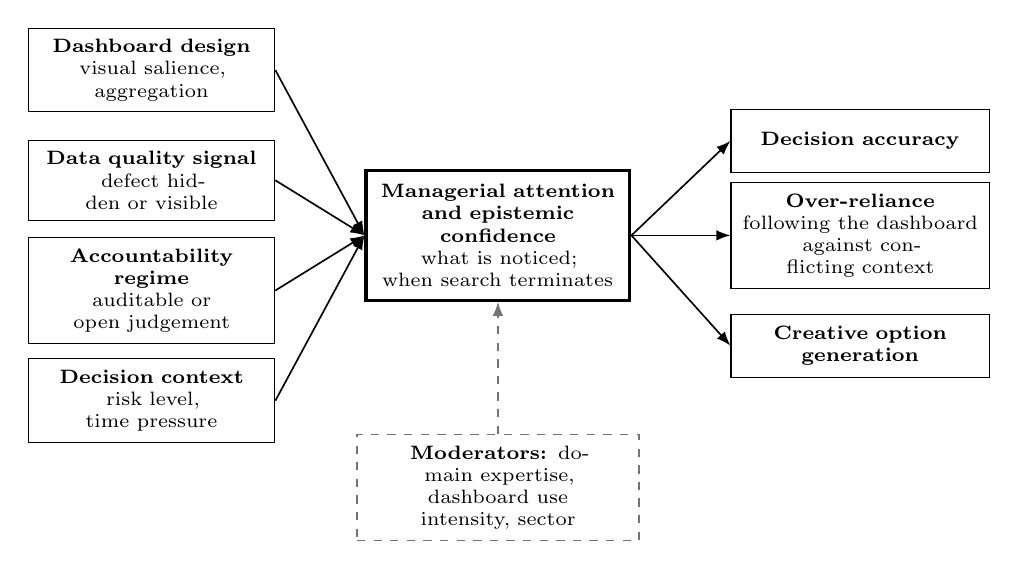
\begin{tikzpicture}[
  every node/.style={font=\scriptsize},
  box/.style={draw=black,align=center,inner sep=4pt,text width=2.85cm,minimum height=0.95cm},
  med/.style={draw=black,line width=1.1pt,align=center,inner sep=5pt,text width=3.0cm,minimum height=1.35cm},
  outc/.style={draw=black,align=center,inner sep=4pt,text width=3.0cm,minimum height=0.8cm},
  mod/.style={draw=black!55,dashed,align=center,inner sep=4pt,text width=3.3cm},
  ar/.style={-{Latex[length=1.8mm]},line width=0.6pt}]
\node[box] (a1) at (0,2.9) {\textbf{Dashboard design}\\visual salience, aggregation};
\node[box] (a2) at (0,1.5) {\textbf{Data quality signal}\\defect hidden or visible};
\node[box] (a3) at (0,0.1) {\textbf{Accountability regime}\\auditable or open judgement};
\node[box] (a4) at (0,-1.3) {\textbf{Decision context}\\risk level, time pressure};
\node[med] (m) at (4.4,0.8) {\textbf{Managerial attention\\and epistemic confidence}\\\scriptsize what is noticed;\\\scriptsize when search terminates};
\node[outc] (o1) at (9.0,2.0) {\textbf{Decision accuracy}};
\node[outc] (o2) at (9.0,0.8) {\textbf{Over-reliance}\\\scriptsize following the dashboard\\\scriptsize against conflicting context};
\node[outc] (o3) at (9.0,-0.6) {\textbf{Creative option\\generation}};
\node[mod] (mo) at (4.4,-2.4) {\textbf{Moderators:} domain expertise,\\dashboard use intensity, sector};
\foreach \x in {a1,a2,a3,a4} \draw[ar] (\x.east) -- (m.west);
\foreach \y in {o1,o2,o3} \draw[ar] (m.east) -- (\y.west);
\draw[ar,black!55,dashed] (mo.north) -- (m.south);
\end{tikzpicture}
\caption{Initial conceptual framework of the study}
\label{fig:framework}
\end{figure}

Four antecedent conditions act upon managerial attention and epistemic confidence, which in turn shape
three decision outcomes. RQ1 addresses the modelled paths, whilst RQ2 explains why the accountability path
operates in the manner that it does. It may be noted here that section 5.2 proposes a revision to this
model in the light of the documentary evidence.

\begin{figure}[H]
\centering
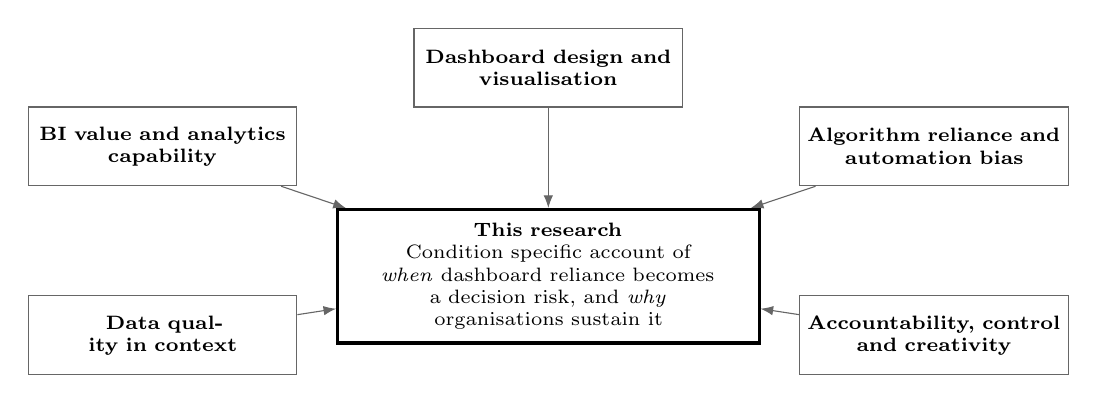
\begin{tikzpicture}[
  every node/.style={font=\scriptsize},
  str/.style={draw=black!60,align=center,inner sep=3pt,text width=3.2cm,minimum height=1.0cm},
  gapb/.style={draw=black,line width=1.1pt,align=center,inner sep=5pt,text width=5.0cm,minimum height=1.4cm},
  ar/.style={-{Latex[length=1.6mm]},black!60}]
\node[str] (s1) at (-4.9,2.9) {\textbf{BI value and analytics\\capability}};
\node[str] (s2) at (0,3.9) {\textbf{Dashboard design and\\visualisation}};
\node[str] (s3) at (4.9,2.9) {\textbf{Algorithm reliance and\\automation bias}};
\node[str] (s4) at (-4.9,0.5) {\textbf{Data quality in context}};
\node[str] (s5) at (4.9,0.5) {\textbf{Accountability, control\\and creativity}};
\node[gapb] (g) at (0,1.25) {\textbf{This research}\\Condition specific account of\\\emph{when} dashboard reliance becomes\\a decision risk, and \emph{why}\\organisations sustain it};
\foreach \x in {s1,s2,s3,s4,s5} \draw[ar] (\x) -- (g);
\end{tikzpicture}
\caption{Map of contributing research streams and the position of this study}
\label{fig:map}
\end{figure}

The study sits at the intersection of the five streams rather than within any single one of them. Its
distinctiveness lies in the joint treatment of design, data quality, accountability and creativity as
conditions bearing upon one behavioural outcome.

\section{Hypotheses}

The experimental strand tests the hypotheses which are set out at Table~\ref{tab:hyp}. It may be noted that
H4 is stated as a pair of competing predictions, since the literature supports both directions, and
establishing which of them obtains in dashboard settings is itself a contribution.

\begin{table}[H]
\centering\small
\caption{Hypotheses, theoretical basis and tested contrast}
\label{tab:hyp}
\begin{tabularx}{\textwidth}{@{}p{0.9cm} X p{4.0cm}@{}}
\toprule
\textbf{ID} & \textbf{Hypothesis} & \textbf{Theoretical basis} \\
\midrule
H1 & Over-reliance is higher when the data quality defect is hidden than when a freshness or completeness
warning is visible. & Wang and Strong (1996); Lyell and Coiera (2017) \\
H2 & Over-reliance is higher when the decision is framed as auditable than as open managerial judgement,
holding the data constant. & Espeland and Sauder (2007); Franco-Santos and Otley (2018) \\
H3 & Decision accuracy is lower where one key performance indicator dominates visually than under a
balanced multi-indicator view. & Cleveland and McGill (1984); Sarikaya et al. (2019) \\
H4a & Higher decision risk \emph{increases} dashboard deference, through a defensibility motive. &
Legitimacy asymmetry, section 2.5 \\
H4b & Higher decision risk \emph{decreases} dashboard deference, through a verification motive. &
Dietvorst, Simmons and Massey (2015) \\
H5 & Dashboard deference is negatively associated with the number of distinct alternative actions
generated. & Amabile (1998); Doshi and Hauser (2024) \\
H6 & Domain expertise moderates H1, such that more experienced managers challenge hidden defect dashboards
more frequently. & Kahneman (2011); Lebovitz, Lifshitz-Assaf and Levina (2022) \\
\bottomrule
\end{tabularx}
\end{table}

%=====================================================================
\chapt{3}{Research Methodology}
%=====================================================================

This chapter sets out the methodology employed in order to address the research questions stated
at section 1.4. It is organised following the layers of the research onion of Saunders, Lewis and
Thornhill (2019), reproduced at Figure~\ref{fig:onion}, and proceeds through research philosophy,
research approach, research strategy, research methods, and data collection. Quality criteria,
ethical considerations and methodological limitations are addressed thereafter.

\begin{figure}[H]
\centering
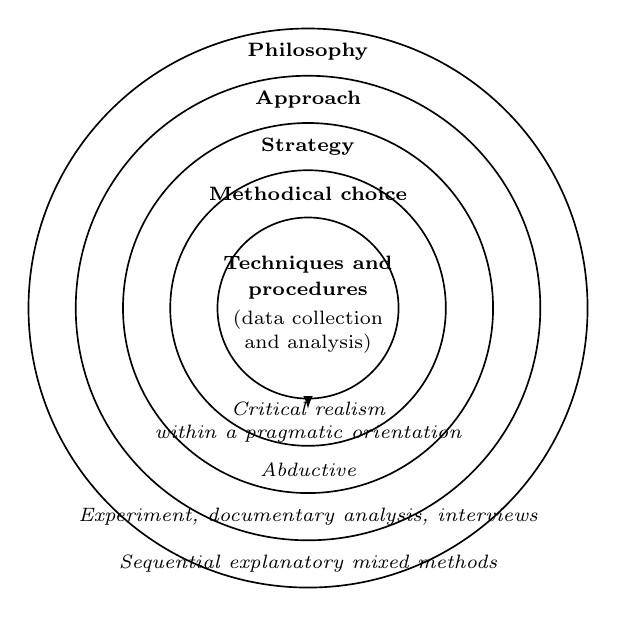
\begin{tikzpicture}[every node/.style={font=\scriptsize}]
\foreach \r/\lbl in {3.55/{}, 2.95/{}, 2.35/{}, 1.75/{}, 1.15/{}}
  \draw[black,line width=0.6pt] (0,0) circle (\r);
\node at (0,3.25) {\textbf{Philosophy}};
\node at (0,2.65) {\textbf{Approach}};
\node at (0,2.05) {\textbf{Strategy}};
\node at (0,1.45) {\textbf{Methodical choice}};
\node at (0,0.55) {\textbf{Techniques and}};
\node at (0,0.22) {\textbf{procedures}};
\node at (0,-0.15) {\scriptsize(data collection};
\node at (0,-0.45) {\scriptsize and analysis)};
\node[align=center] at (0,-1.45) {\itshape Critical realism\\\itshape within a pragmatic orientation};
\node[align=center] at (0,-2.05) {\itshape Abductive};
\node[align=center] at (0,-2.65) {\itshape Experiment, documentary analysis, interviews};
\node[align=center] at (0,-3.25) {\itshape Sequential explanatory mixed methods};
\draw[-{Latex[length=1.6mm]},line width=0.6pt] (0,-1.15) -- (0,-1.28);
\end{tikzpicture}
\caption{Layers of the research onion as applied in this study, after Saunders, Lewis and Thornhill (2019)}
\label{fig:onion}
\end{figure}

\section{Research philosophy: critical realism within a pragmatic orientation}

The study adopts a critical realist ontology within a pragmatic orientation. Decision errors and
their organisational consequences are treated as real and consequential independently of how they
are described, whilst the mechanisms which produce them, namely legitimacy, defensibility and
professional risk, are socially constituted and accessible only through interpretation. This
stratified view of reality, in which observable events are generated by underlying mechanisms
which may or may not be actualised (Bhaskar, 2008), suits a study whose central construct is a mechanism rather than a variable. Positivism was
rejected because it would capture the experimental strand but could not accommodate legitimacy,
which is neither directly observable nor stable across settings. Interpretivism was rejected as a
sole position because it would capture RQ2 but would forbid the controlled comparison which RQ1
requires. A full comparison of the positions considered is placed at Appendix~B, and pragmatism is
adopted as the practical orientation, following established mixed methods guidance (Creswell and
Plano Clark, 2018; Tashakkori and Teddlie, 2010).

\section{Research approach: abductive}

The study reasons abductively. Theory specifies the initial conditions and the hypotheses, and
empirical patterns thereafter refine the framework (Saunders, Lewis and Thornhill, 2019). A purely
deductive approach would require the framework to be settled in advance and merely tested,
forfeiting the chief benefit of running the documentary strand first. A purely inductive approach
would forfeit the hypotheses which make the experimental strand interpretable. Section 5.2 is an
instance of abduction in operation, since the documentary evidence has required the framework to
be amended rather than merely confirmed.

\section{Research strategy: sequential explanatory mixed methods}

\subsection{Design alternatives considered and rejected}

A defensible methodology requires justification not only of what was done but equally of what was not done.
Table~\ref{tab:alt} accordingly records the principal alternatives which were considered.

\begin{table}[H]
\centering\footnotesize
\caption{Design alternatives considered and the basis for rejection}
\label{tab:alt}
\begin{tabularx}{\textwidth}{@{}p{3.4cm} X@{}}
\toprule
\textbf{Alternative} & \textbf{Basis for rejection} \\
\midrule
Field experiment within a single organisation & Strongest ecological validity, but requires gatekeeper
access to live decision systems, raises acute commercial confidentiality risk, and would confound the
accountability manipulation with the culture of a single firm. Not feasible within the timetable. \\
Cross sectional survey of attitudes towards dashboards & Measures stated beliefs rather than decision
behaviour, and is exposed to common method bias where predictors and outcome are self reported from a single
instrument (Podsakoff et al., 2003). The construct of interest is behaviour under conflicting evidence,
which a survey cannot observe. \\
Single in-depth organisational case study & Well suited to mechanism identification (Eisenhardt, 1989; Yin,
2018) but incapable of establishing the conditional variation which RQ1 requires, since conditions cannot be
varied within one setting. \\
Interviews alone & Would answer RQ2 but not RQ1, and would rely upon retrospective self report concerning a
behaviour which participants have little incentive to recall accurately. \\
Secondary analysis of an existing dataset & No public dataset records dashboard level decision episodes
together with the contextual evidence available at the time. \\
\midrule
\textbf{Adopted: sequential explanatory mixed methods with a concurrent documentary strand} & Experimental
vignettes vary condition whilst holding the decision maker constant. Documentary analysis anchors the
mechanism in real organisational outcomes. Interviews explain the observed behaviour. Each strand
compensates for a specific weakness in the others, as section 3.6 sets out. \\
\bottomrule
\end{tabularx}
\end{table}

The adopted design is depicted at Figure~\ref{fig:design}. Strand 2 was run first for the reason that it
requires neither ethical approval nor recruitment, and its failure patterns sharpen the interview protocol.

\begin{figure}[H]
\centering
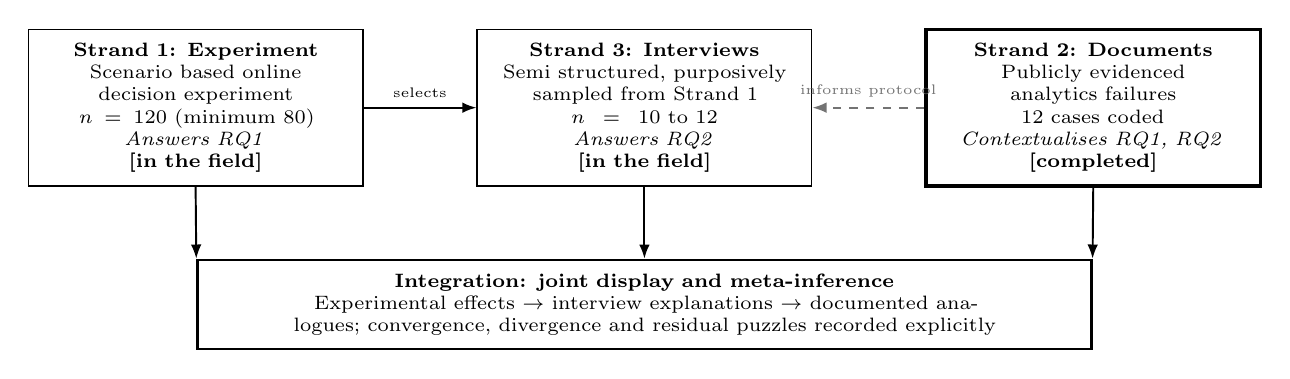
\begin{tikzpicture}[
  every node/.style={font=\scriptsize},
  ph/.style={draw=black,align=center,inner sep=5pt,text width=3.9cm,minimum height=1.6cm},
  done/.style={draw=black,line width=1.2pt,align=center,inner sep=5pt,text width=3.9cm,minimum height=1.6cm},
  jd/.style={draw=black,line width=0.9pt,align=center,inner sep=5pt,text width=11.0cm},
  ar/.style={-{Latex[length=1.8mm]},line width=0.7pt}]
\node[ph] (p1) at (0,0) {\textbf{Strand 1: Experiment}\\Scenario based online\\decision experiment\\$n = 120$ (minimum 80)\\\emph{Answers RQ1}\\\textbf{[in the field]}};
\node[ph] (p3) at (5.7,0) {\textbf{Strand 3: Interviews}\\Semi structured, purposively\\sampled from Strand 1\\$n = 10$ to $12$\\\emph{Answers RQ2}\\\textbf{[in the field]}};
\node[done] (p2) at (11.4,0) {\textbf{Strand 2: Documents}\\Publicly evidenced\\analytics failures\\12 cases coded\\\emph{Contextualises RQ1, RQ2}\\\textbf{[completed]}};
\node[jd] (j) at (5.7,-2.5) {\textbf{Integration: joint display and meta-inference}\\\scriptsize Experimental effects $\rightarrow$ interview explanations $\rightarrow$ documented analogues; convergence, divergence and residual puzzles recorded explicitly};
\draw[ar] (p1) -- node[above,font=\tiny]{selects} (p3);
\draw[ar,black!55,dashed] (p2) -- node[above,font=\tiny]{informs protocol} (p3);
\draw[ar] (p1.south) -- (j.north west);
\draw[ar] (p3.south) -- (j.north);
\draw[ar] (p2.south) -- (j.north east);
\end{tikzpicture}
\caption{Sequential explanatory design with a concurrent documentary strand}
\label{fig:design}
\end{figure}

\subsection{Mapping of research questions to methods}

Table~\ref{tab:matrix} maps each research question onto the method, the data source, the intended analysis
and the expected output. This mapping was prepared before data collection commenced and has not been
altered since.

\begin{table}[H]
\centering\footnotesize
\caption{Mapping of research questions to method, data source, analysis and expected output}
\label{tab:matrix}
\begin{tabularx}{\textwidth}{@{}p{1.2cm} p{2.3cm} X p{2.6cm} p{2.6cm}@{}}
\toprule
\textbf{RQ} & \textbf{Method} & \textbf{Data source} & \textbf{Analysis} & \textbf{Expected output} \\
\midrule
RQ1a & Scenario experiment (Strand 1) & 120 professionals $\times$ 4 vignettes, approximately 480 decision
observations & Mixed effects logistic regression; odds ratios with 95\% CI & Condition specific
probabilities of deference \\
RQ1b & Same instrument, count outcome & Number of distinct alternative actions per vignette & Poisson or
negative binomial regression & Estimate of option-set narrowing \\
RQ1 (context) & Documentary analysis (Strand 2) & Regulator notices, inquiry and royal commission reports &
Structured extraction; cross-case matrix & Comparative failure pattern matrix \textbf{[complete]} \\
RQ2a & Semi structured interviews (Strand 3) & 10 to 12 professionals selected on Strand 1 behaviour &
Reflexive thematic analysis & Mechanism themes for deference and challenge \\
RQ2b & Interviews and documents & Interview accounts triangulated against control failures & Pattern
matching across strands & Conditions enabling challenge; governance framework \\
\bottomrule
\end{tabularx}
\end{table}

\section{Research methods: mixed method}

Both quantitative and qualitative methods are employed. The quantitative component, being the
scenario experiment, generates numerical data upon decision behaviour under systematically varied
conditions and is therefore suited to the conditional question posed at RQ1. The qualitative
components, being the documentary analysis and the interviews, generate rich accounts of the
mechanisms behind the observed behaviour and are suited to the explanatory question posed at RQ2.
Neither component is subordinate to the other. The design is genuinely mixed rather than
quantitative work with qualitative illustration appended to it, and the integration procedure is
stated at section 4.5.

\section{Data collection}

\subsection{Strand 1: scenario based decision experiment}

\textbf{\emph{Instrument design.}} The instrument follows established experimental vignette methodology,
which is well suited to the examination of judgement and decision making in circumstances where the factors
of interest cannot ethically or practically be manipulated in the field (Aguinis and Bradley, 2014;
Atzmüller and Steiner, 2010). The design is a $2\times2\times2$ within-subjects vignette experiment. Each
vignette presents a realistic dashboard image together with a short decision brief containing a contextual
cue which conflicts with the headline signal of the dashboard. By way of example, a supply chain dashboard
may show demand as being stable whilst a named regional depot reports repeated delivery failures. The
factors and the measures are set out at Table~\ref{tab:factors}. A copy of the instrument is placed at
Appendix~H.

Two design decisions follow directly from the appraisal at section 2.7. Participants are
practising professionals rather than students, which addresses the ecological validity concern,
and accountability framing is manipulated explicitly rather than held constant, which addresses
the omission that makes generic advice taking studies difficult to transfer.

\begin{table}[H]
\centering\footnotesize
\caption{Experimental factors, levels and operationalisation}
\label{tab:factors}
\begin{tabularx}{\textwidth}{@{}p{3.0cm} p{3.1cm} X@{}}
\toprule
\textbf{Factor} & \textbf{Levels} & \textbf{Operationalisation} \\
\midrule
Decision risk & High or Low & Stated financial and reputational consequence of an incorrect decision \\
Data quality signal & Hidden or Visible & Presence or absence of a banner disclosing that the feed is six
days stale and twelve per cent incomplete \\
Accountability framing & Auditable or Open judgement & Instruction that the decision will be recorded and
reviewed against the dashboard, as against being recorded as a managerial judgement \\
Metric salience \emph{(between subjects)} & Single dominant KPI or Balanced multi-indicator & Visual
emphasis manipulated through size and position \\
\midrule
\multicolumn{3}{@{}l}{\textbf{Measured outcomes}}\\
Over-reliance \emph{(primary)} & Binary & Chose the dashboard consistent action despite the conflicting
contextual cue \\
Decision accuracy & Binary & Chose the action which is correct on all available evidence \\
Creative option generation & Count & Number of distinct alternative actions listed, double coded \\
Confidence & Seven point scale & Self rated confidence in the chosen action \\
Verification intent & Binary & Whether additional data were requested before deciding \\
\midrule
\multicolumn{3}{@{}l}{\textbf{Covariates:} sector, years of experience, seniority, dashboard use frequency,
self rated analytics familiarity}\\
\bottomrule
\end{tabularx}
\end{table}

\textbf{\emph{The sample.}} Participants are working professionals who use dashboards, key performance
indicator reports or business intelligence tools in a managerial or analytical capacity, in finance,
consulting, operations, logistics, technology or analytics roles. Recruitment is non-probability purposive
with snowball extension. A screening question enforces the inclusion criterion of dashboard use at least
weekly during the preceding twelve months.

\nbox{Sample size justification}{%
\textbf{Target $N = 120$ completed responses; minimum viable $N = 80$.} Each participant completes four of
eight vignettes, randomised and counterbalanced, which yields approximately 480 decision observations at the
target. For a two-proportion comparison of over-reliance rates of 0.35 against 0.60 at $\alpha = .05$
(two-tailed) and power of $.80$, approximately 123 independent observations are required (Cohen, 1988;
Field, 2018). Since the design is within-subjects, the effective requirement is inflated by the design
effect $1+(m-1)\rho$. At $m=4$ and an intra-class correlation of $\rho = .20$ the design effect is 1.60,
which implies roughly 50 participants for that single contrast. The target of 120 therefore provides margin
to detect differences of approximately 20 percentage points, to estimate the three-way condition structure
rather than a single contrast, and to test the expertise moderation at H6.}

\textbf{\emph{Piloting and analysis.}} The instrument is piloted with eight to ten respondents
from the target population together with two academic reviewers, checking that the contextual cue
is noticed without dominating, that the data quality banner is legible without becoming a demand
characteristic, that completion time remains under twelve minutes, and that double coding of the
creativity count is reliable. Attention checks, a minimum time filter and manipulation checks
guard against inattentive responding and failed manipulation. The primary model is a mixed effects
logistic regression with a random intercept for participant, predicting over-reliance from
decision risk, data quality signal, accountability framing, metric salience and the pre-specified
interactions. Alternative option counts are modelled by Poisson or negative binomial regression
with overdispersion tested. Where the assumptions of the mixed model cannot be satisfied, the
pre-committed fallback is logistic regression with cluster robust standard errors, supplemented by
McNemar tests for within-subject paired contrasts. Effect sizes are reported alongside
significance values, and the analysis plan was fixed before data collection in order to prevent
selective reporting.

\subsection{Strand 2: documentary analysis}

\textbf{\emph{Rationale and admissibility.}} Documentary analysis is appropriate in circumstances where the
phenomenon of interest leaves a durable and independently verifiable trace, and where the researcher cannot
be present at the events concerned (Bowen, 2009; Krippendorff, 2018). Both conditions hold in the present
case, since organisational analytics failures of consequence generate statutory investigation, and no
researcher could possibly observe such an episode as it unfolds.

Only documents whose independent existence may be verified are admissible. These comprise
regulator enforcement notices and consent orders; statutory public inquiry and royal commission
reports; independent reviews commissioned by regulators; national audit office and parliamentary
committee reports; and listed company annual reports and restatement disclosures. Press coverage
may be used to locate a case but never as the sole evidential basis for a coded judgement. Cases
were selected by maximum variation sampling across sector and failure type so as to avoid an
all-finance sample, subject to the requirements that the event occurred between 2010 and 2026,
that primary documentation is available in English, and that the facts are settled rather than
contested in ongoing proceedings.

\textbf{\emph{Evidential grading and coding reliability.}} A refinement adopted during coding, and
one not commonly reported at this level, is the explicit grading of evidential strength. Grade A
denotes a case documented by a dedicated statutory investigation, royal commission or regulatory
enforcement notice. Grade B denotes a case documented by official organisational disclosure
together with parliamentary or regulatory scrutiny but without a dedicated independent
investigation. Of the twelve cases, ten are Grade A and two are Grade B. The grading is reported
transparently so that a reader may discount the weaker cases.

Each case was coded against the fixed frame which is set out at Table~\ref{tab:frame}, with a verbatim
supporting quotation and page reference recorded for every judgement. A second coder independently coded a
thirty per cent subsample. Agreement will be reported as Cohen's $\kappa$ (Cohen, 1960) and interpreted
against the conventional benchmarks (Landis and Koch, 1977), with disagreements resolved by discussion and
the resolution logged.

\begin{table}[H]
\centering\small
\caption{Structured extraction frame for the documentary analysis}
\label{tab:frame}
\begin{tabularx}{\textwidth}{@{}p{3.4cm} X@{}}
\toprule
\textbf{Dimension} & \textbf{Coded content} \\
\midrule
Failure type & Accuracy, timeliness, completeness, consistency or model logic \\
Signal visibility & Was the defect detectable from the interface or report at the point of use? Coded as
silent, partial or visible \\
Detection lag & Elapsed time between failure onset and organisational recognition \\
Human challenge & Was the output challenged? By whom? Was the challenge escalated, ignored or overridden? \\
Legitimacy asymmetry & Evidence that system output was treated as more authoritative than human accounts;
coded as strong, moderate or weak \\
Control mechanism & Warnings, overrides, reconciliation or governance which existed, and the reason for
their failure \\
Organisational impact & Financial, operational, regulatory and human consequences \\
Evidential grade & A or B, as defined above \\
\bottomrule
\end{tabularx}
\end{table}

\subsection{Strand 3: semi structured interviews}

Ten to twelve interviews will be conducted, with a floor of eight, which reflects the evidence that
thematic saturation in relatively homogeneous samples typically emerges within approximately twelve
interviews (Guest, Bunce and Johnson, 2006) whilst remaining feasible within the timetable (Bryman, 2016).

Participants are selected purposively from those Strand 1 respondents who consent to follow-up, and they
are sampled upon \emph{observed behaviour} rather than upon convenience. Three behavioural profiles are
sought, namely strong deference across conditions, consistent challenge behaviour, and inconsistent
response to data quality warnings. This behaviour linked sampling is the mechanism which makes the design
genuinely explanatory rather than merely sequential, since it permits the interview to interrogate a
specific decision which the participant actually made rather than a decision which he or she reports having
made. Interviews last thirty to forty minutes and are conducted online. Analysis follows reflexive thematic
analysis (Braun and Clarke, 2006), with NVivo supporting coding, memoing and theme development. The
interview guide is placed at Appendix~E.

\section{Quality criteria}

Quantitative and qualitative criteria are treated separately, following the usual convention
(Lincoln and Guba, 1985; Saunders, Lewis and Thornhill, 2019). For Strand 1, internal validity
rests upon randomised and counterbalanced vignette allocation within a within-subjects design,
construct validity upon double coding and pilot testing of cue salience, and protection against
common method bias upon the fact that the outcome is a behavioural choice whilst the predictors
are manipulated rather than measured (Podsakoff et al., 2003). For Strand 2, authenticity rests
upon the admissibility rule and the evidential grading, and reliability upon the fixed extraction
frame and thirty per cent double coding. For Strand 3, credibility rests upon behaviour linked
sampling and member checking, dependability upon an audit trail of coding decisions, and
transferability upon thick description of sector and role. As a matter of reflexivity, the
analytics training of the researcher creates a plausible bias towards reading deference as error,
and the coding therefore actively seeks accounts in which deference proved correct. The full
mapping of criteria to actions is placed at Appendix~C.

\section{Ethical considerations}

Ethical approval, the fieldwork risk assessment and the GDPR assessment were completed and approved before
any primary data collection commenced, in accordance with the University Code of Good Practice in Research.
The study is additionally conducted in accordance with the MRS Code of Conduct (Market Research Society,
2019), whose provisions on informed consent, non-deception and the avoidance of harm apply directly to
research with professional participants. Four design specific matters warrant particular mention.

\textbf{\emph{Participants must not be made to feel personally evaluated.}} The experiment
presents decision problems having better and worse answers, and the participants are professionals
whose competence forms part of their identity. The study is therefore framed throughout as
research into how dashboards are designed and used, and never into individual managerial ability.
No participant receives a score, no individual level feedback is given, and results are reported
only in the aggregate. The debrief explains that the scenarios were deliberately constructed so
that the dashboard could mislead, and that following it was accordingly reasonable rather than
incompetent. Some concealment of the manipulation is unavoidable if the behaviour is to be
observed at all, and this is handled by full disclosure at debrief rather than by active deception
at any point.

\textbf{\emph{Commercial confidentiality and professional risk.}} Interviewees work in regulated, client
facing or commercially sensitive environments. The information sheet and the verbal preamble state
explicitly that participants must not disclose confidential organisational information, proprietary
dashboard designs, client data, named clients or commercially sensitive decision processes. Should a
participant begin to disclose any such material, the interviewer will interrupt and the passage will be
excluded from transcription. Employers are described by sector and size band only.

\textbf{\emph{Data protection.}} Data are held upon University provided encrypted storage,
transcripts are pseudonymised at the point of transcription, recordings are deleted following
verification, and processing is on the basis of consent under the UK GDPR. Participants may
withdraw without giving any reason and may request deletion of their data up to two weeks after
participation, after which anonymisation renders retrieval impossible.

\textbf{\emph{Secondary data and the dignity of those harmed.}} Strand 2 uses only material which is
already in the public domain. Since several of the cases involve identifiable individuals who suffered
serious harm, the Post Office and Robodebt cases being the most obvious instances, the analysis focuses
upon organisational and system level control failures rather than upon individual conduct, and it treats
human consequences with proportionate care rather than as illustrative colour.

\section{Methodological limitations}

Four limitations are stated explicitly, in keeping with the expectation that limitations be made explicit
rather than merely implied.

Firstly, the vignette design measures stated decisions in a low stakes setting. However realistic
the dashboard, no participant loses money or standing by choosing wrongly, and the accountability
manipulation is therefore a simulation of accountability rather than the thing itself. The
resulting bias runs towards understating deference, since the defensibility motive is weaker in
the laboratory than in the organisation. Secondly, non-probability recruitment limits
generalisation, and self selection may over-represent professionals already reflective about
analytics. Sector and seniority distributions will be reported transparently rather than claimed
to be representative. Thirdly, the documentary strand is subject to severe survivorship bias,
discussed at section 5.3. It establishes the anatomy of failure and not its base rate. Fourthly,
the three strands are not equally weighted in evidential strength. The documentary strand rests
upon authoritative primary documents but a small purposive sample, the experimental strand upon a
larger sample but an artificial task, and the interview strand upon rich accounts but
retrospective self report. Integration must therefore be interpretive rather than arithmetic, and
no strand is treated as validating another in any strong sense.

%=====================================================================
\chapt{4}{Findings}
%=====================================================================

\section{Overview}

This chapter presents the findings of the study. The documentary strand has been completed in full and is
reported at section 4.2. The experimental and interview strands remain in the field at the date of this
draft, and sections 4.3 and 4.4 are accordingly left blank and marked. Section 4.5 sets out the joint
display through which the three strands will be integrated once all of them have reported.

\section{Strand 2: documentary analysis of twelve organisational failures}

\subsection{The case sample}

Twelve cases satisfied the inclusion criteria and were coded in full, spanning nine sectors and four
jurisdictions, as set out at Table~\ref{tab:cases}. Every case is anchored to a document whose independent
existence may be verified, in accordance with the admissibility rule stated at section 3.5.2.

\begin{table}[H]
\centering\footnotesize
\caption{The documentary case sample, with evidential grade and primary source}
\label{tab:cases}
\begin{tabularx}{\textwidth}{@{}p{0.7cm} p{2.9cm} p{2.5cm} p{1.5cm} p{0.7cm} X@{}}
\toprule
\textbf{ID} & \textbf{Case} & \textbf{Sector} & \textbf{Period} & \textbf{Gr.} & \textbf{Primary source} \\
\midrule
C1 & Post Office Horizon & Postal and retail (UK) & 1999--2019 & A & Post Office Horizon IT Inquiry (2025), Vol. 1 \\
C2 & NATS flight planning & Aviation (UK) & 2023 & A & Civil Aviation Authority (2024), CAP2993 \\
C3 & Citibank risk data & Banking (US) & 2013--2020 & A & Office of the Comptroller of the Currency (2020), NR 2020-132 \\
C4 & PHE case undercount & Public health (UK) & 2020 & B & Official statements and parliamentary scrutiny (2020) \\
C5 & Robodebt & Welfare (AU) & 2015--2020 & A & Royal Commission into the Robodebt Scheme (2023) \\
C6 & TSB migration & Banking (UK) & 2018 & A & Financial Conduct Authority (2022), Final Notice \\
C7 & Knight Capital & Trading (US) & 2012 & A & Securities and Exchange Commission (2013), Order 34-70694 \\
C8 & Ofqual grading & Education (UK) & 2020 & A & Office for Statistics Regulation (2021) \\
C9 & Dutch childcare benefits & Welfare and tax (NL) & 2013--2020 & A & Autoriteit Persoonsgegevens (2021) \\
C10 & Goldman Sachs reporting & Banking (UK) & 2007--2017 & A & Financial Conduct Authority (2019), Final Notice \\
C11 & Zillow Offers & Real estate and technology (US) & 2021 & B & Zillow Group (2021), Q3 shareholder letter \\
C12 & Boeing 737 MAX (MCAS) & Aerospace (US) & 2012--2019 & A & US House Committee on Transportation and Infrastructure (2020) \\
\bottomrule
\end{tabularx}
\end{table}

\subsection{Failure types and visibility of the defect}

Figure~\ref{fig:failtype} presents the distribution of failure types, disaggregated by whether the defect
was detectable at the point of use. Two observations follow from it.

Firstly, model logic failures dominate, accounting for eight of the twelve cases. The problem was
most commonly not that a number had been entered wrongly, but rather that the system was doing
exactly what it had been designed to do upon a rule which was itself inappropriate for the
situation. Robodebt is the clearest illustration, since averaging annual income across fortnightly
periods was arithmetically faultless and at the same time substantively wrong for any person whose
earnings varied across the year (Royal Commission into the Robodebt Scheme, 2023). The Ofqual
standardisation model of 2020 likewise executed its specification correctly whilst producing
outcomes which could not be defended at the level of the individual pupil (Office for Statistics
Regulation, 2021).

Secondly, and of greater importance for the argument advanced here, the defect was silent at the point of
use in seven cases and only partially visible in a further four. In one case only, being the TSB migration of
2018, where customers were immediately unable to access their accounts, was the failure plainly visible to
those affected (Financial Conduct Authority, 2022). This provides direct documentary support for the
premise stated at section 2.4, namely that data and model defects do not announce themselves.

\begin{figure}[H]
\centering

\includegraphics[width=0.86\textwidth]{fig/f_failtype.pdf}
\caption{Distribution of failure types across the twelve cases, disaggregated by visibility of the defect
at the point of use}
\label{fig:failtype}
\end{figure}

\subsection{Detection lag and the cost of silence}

If a defect gives no perceptual cue, one would naturally expect it to persist. Figure~\ref{fig:lag} plots
detection lag upon a logarithmic scale, shaded by signal visibility, and Figure~\ref{fig:box} summarises
the same relationship.

The pattern is stark. Cases in which the defect was silent persisted for a median of several years. Post
Office Horizon persisted for approximately sixteen years (Post Office Horizon IT Inquiry, 2025). The
transaction reporting failures of Goldman Sachs International persisted for some nine and a half years,
covering approximately 213.6 million reportable transactions (Financial Conduct Authority, 2019). The Dutch
childcare benefits risk classification persisted for around seven years (Autoriteit Persoonsgegevens,
2021). The manoeuvring characteristics augmentation system of the Boeing 737 MAX persisted for roughly six
years from specification to the second accident (US House Committee on Transportation and Infrastructure,
2020). By way of contrast, cases which produced a perceptible signal were recognised within hours or days.
Knight Capital was recognised within approximately forty-five minutes (Securities and Exchange Commission,
2013), the NATS flight planning failure within a few hours (Civil Aviation Authority, 2024), and the Public
Health England case undercount within roughly eight days.

Care is nonetheless required regarding what this comparison actually shows. The two groups differ
in more than signal visibility alone, since silent defects tend to arise in slower moving
administrative processes whereas signalled defects arise in real time operational systems, and
exposure time is therefore confounded with visibility. The comparison is accordingly suggestive
rather than causal, and no significance test is offered upon twelve purposively selected cases,
the sampling strategy having been designed for variation and not for representativeness. What may
fairly be said is that the record is entirely consistent with the proposition that visibility
governs the speed of correction, and that the proposition is worth testing experimentally, which
is precisely what H1 does.

\begin{figure}[H]
\centering

\includegraphics[width=0.92\textwidth]{fig/f_lag.pdf}
\caption{Detection lag by case, ordered from shortest to longest and shaded by visibility of the defect}
\label{fig:lag}
\end{figure}

\begin{figure}[H]
\centering

\includegraphics[width=0.55\textwidth]{fig/f_box.pdf}
\caption{Detection lag for silent as against partially or fully signalled defects, with individual cases
overlaid}
\label{fig:box}
\end{figure}

\subsection{The principal finding: challenge was raised and overridden}

The most consequential finding of this strand concerns not detection but rather authority.

In nine of the twelve cases a human being challenged the system output, and the challenge was thereafter
overridden, ignored or not acted upon. In one case only, being the decision of Zillow to wind down its
iBuying operation once forecasting losses became apparent, was a challenge raised and acted upon in a
manner which limited the harm (Zillow Group, 2021). In two cases no challenge was raised at all, and in
both of those the defect was entirely silent, so that there was nothing for anybody to challenge.

Figure~\ref{fig:challenge} presents this distribution cross-tabulated with the coded strength of legitimacy
asymmetry. It is notable that every case coded as exhibiting a strong asymmetry falls within the group in
which challenge was raised and overridden.

The qualitative texture of these overrides is instructive. Sub-postmasters challenged the Horizon
figures consistently over many years, and the response was prosecution rather than investigation
(Post Office Horizon IT Inquiry, 2025). In the Robodebt scheme, internal legal advice questioning
the lawfulness of income averaging was obtained and thereafter set aside (Royal Commission into
the Robodebt Scheme, 2023). Engineering concerns regarding the reliance of the 737 MAX system upon
a single angle of attack sensor were raised internally without altering the certification outcome
(US House Committee on Transportation and Infrastructure, 2020). Knight Capital is instructive in
a different manner, in that the systems of the firm generated ninety-seven automated email
messages within the relevant window, but these were not designed as system alerts and were not
treated as such (Securities and Exchange Commission, 2013). The information was present. The
authority to act upon it was not.

This is precisely the pattern which legitimacy asymmetry predicts. The binding constraint upon correction
was not the availability of contrary information but rather the relative institutional standing of the
system output as against the human objection.

\begin{figure}[H]
\centering

\includegraphics[width=0.86\textwidth]{fig/f_challenge.pdf}
\caption{Outcome of human challenge across the twelve cases, cross-tabulated with the coded strength of
legitimacy asymmetry}
\label{fig:challenge}
\end{figure}

\subsection{Cross-case matrix}

Table~\ref{tab:coded} presents the full coded matrix and Figure~\ref{fig:heat} renders the same information
visually. Reading the heat map column by column, it emerges that the cases which produced the gravest human
consequences, namely Horizon, Robodebt, the Dutch childcare benefits scheme and the 737 MAX, share a common
signature, being a silent defect, a strong legitimacy asymmetry, suppressed challenge and a control
mechanism which was either absent or bypassed. This four-way co-occurrence is the empirical shape of the
mechanism which section 2.5 describes theoretically.

\begin{table}[H]
\centering\footnotesize
\caption{Cross-case coded matrix for the documentary strand}
\label{tab:coded}
\begin{tabularx}{\textwidth}{@{}p{0.7cm} p{1.9cm} p{1.4cm} p{1.2cm} X p{1.5cm} p{2.4cm}@{}}
\toprule
\textbf{ID} & \textbf{Failure type} & \textbf{Signal} & \textbf{Lag} & \textbf{Human challenge} &
\textbf{Asym.} & \textbf{Control} \\
\midrule
C1 & Model logic & Silent & 16 yr & Raised, overridden & Strong & Present, ineffective \\
C2 & Model logic & Partial & $\sim$4 hr & Raised, slow escalation & Moderate & Present, ineffective \\
C3 & Consistency & Silent & 7 yr & Raised, overridden & Moderate & Present, ineffective \\
C4 & Completeness & Silent & 8 d & Not raised & Moderate & Absent \\
C5 & Model logic & Silent & 5 yr & Raised, overridden & Strong & Present, bypassed \\
C6 & Consistency & Visible & 1 d & Raised, overridden & Weak & Present, ineffective \\
C7 & Model logic & Partial & $<$2 hr & Alerts issued, ignored & Weak & Absent \\
C8 & Model logic & Partial & 4 d & Raised, overridden & Strong & Present, ineffective \\
C9 & Model logic & Silent & 7 yr & Raised, overridden & Strong & Absent \\
C10 & Accuracy & Silent & 9 yr & Not raised & Weak & Present, ineffective \\
C11 & Model logic & Partial & 6 mo & Raised, acted upon & Moderate & Present, effective \\
C12 & Model logic & Silent & 6 yr & Raised, overridden & Strong & Present, bypassed \\
\bottomrule
\end{tabularx}
\end{table}

\begin{figure}[H]
\centering

\includegraphics[width=0.78\textwidth]{fig/f_heat.pdf}
\caption{Cross-case heat map of the four principal coded dimensions, where H denotes high, M moderate and L
low}
\label{fig:heat}
\end{figure}

\subsection{Control mechanisms and the reasons for their failure}

In one case only was a control mechanism both present and effective. In six cases a control
existed but proved ineffective, in two it existed and was bypassed, and in three it was absent
altogether. The Public Health England undercount is particularly illuminating, because the missing
control was so elementary. No reconciliation was performed as between the number of records
dispatched and the number received, and consequently a silent truncation at the row limit of an
obsolete file format passed unnoticed for roughly a week.

The wider lesson, which the governance framework at section 6.2 must accommodate, is that the controls
which failed were overwhelmingly \emph{detective} in character rather than \emph{authorising}.
Organisations possessed mechanisms for spotting problems. What they generally lacked was any mechanism
conferring standing upon the person who had in fact spotted one.

\section{Strand 1: experimental findings}

\blankbox{awaiting Strand 1 data collection}{%
This section will report the scenario based decision experiment described at section 3.5.1. The structure
has been fixed in advance of data collection, and the analysis script has been written and tested so that
only execution remains. No result is stated here, and nothing has been estimated or simulated in place of
the data.\\[6pt]
\textbf{4.3.1 Sample and data screening.} Response and completion rates; exclusions for failed attention
checks and sub-threshold completion times; final analytic $N$; and participant profile by sector, seniority
and dashboard use frequency.\\[4pt]
\textbf{4.3.2 Descriptive results.} Over-reliance and accuracy rates by experimental condition, with a
grouped bar chart across the eight vignette cells and a histogram of alternative option counts.\\[4pt]
\textbf{4.3.3 Hypothesis tests.} Mixed effects logistic regression of over-reliance upon decision risk,
data quality signal, accountability framing and metric salience, reported as odds ratios with 95 per cent
confidence intervals and a forest plot. H1, H2, H3 will be reported here, and H4a and H4b will be
adjudicated.\\[4pt]
\textbf{4.3.4 Option generation.} Count model of the alternatives generated, testing H5.\\[4pt]
\textbf{4.3.5 Moderation by expertise.} Test of H6 as an interaction term, with a marginal effects plot.}

\section{Strand 3: interview findings}

\blankbox{awaiting Strand 3 data collection}{%
This section will report the reflexive thematic analysis of the semi structured interviews described at
section 3.5.3. Sampling depends upon Strand 1 behaviour and therefore cannot commence until Strand 1 has
closed.\\[6pt]
\textbf{4.4.1 Participant profile.} Sector, role, seniority and the Strand 1 behavioural profile upon which
each participant was selected, presented in pseudonymised form.\\[4pt]
\textbf{4.4.2 Themes.} Four to six named themes with illustrative quotations and a thematic map. The
anticipated themes, held loosely and open to disconfirmation, are defensibility, verification cost,
suppressed intuition, permission to challenge, and the measured option.\\[4pt]
\textbf{4.4.3 Disconfirming accounts.} Instances in which deference proved to be correct and challenge would
have been mistaken, reported explicitly rather than set aside.}

\section{Integration across the three strands}

\blankbox{awaiting Strands 1 and 3}{%
The three strands will be integrated through the joint display at Table~\ref{tab:joint}, of which the first
column is already populated from the completed documentary strand. Divergences between the strands will be
recorded rather than smoothed away. The provisional meta-inferences stated in the final column are
hypotheses awaiting test and are not findings.}

\begin{table}[H]
\centering\footnotesize
\caption{Joint display for integration, with the documentary column populated and the remainder pending}
\label{tab:joint}
\begin{tabularx}{\textwidth}{@{}p{3.4cm} p{3.2cm} p{3.2cm} X@{}}
\toprule
\textbf{Documented pattern (Strand 2, complete)} & \textbf{Experimental finding (Strand 1, pending)} &
\textbf{Explanation (Strand 3, pending)} & \textbf{Provisional meta-inference} \\
\midrule
Silent defects persisted for years, whilst signalled defects were caught within days & \emph{H1:
over-reliance higher when the defect is hidden} & \emph{Why practitioners treat absence of warning as
assurance} & Absence of a warning appears to be read as positive assurance rather than as absence of
information \\
\addlinespace
Challenge was raised and overridden in nine of twelve cases & \emph{H2: auditable framing raises deference}
& \emph{Whether defensibility is the stated reason} & Legitimacy asymmetry may operate at both the
individual and the institutional level \\
\addlinespace
Controls were detective rather than authorising & \emph{Verification intent by condition} & \emph{Conditions
under which challenge is permitted} & Governance may need to confer standing, and not merely detection
capability \\
\bottomrule
\end{tabularx}
\end{table}

%=====================================================================
\chapt{5}{Discussion}
%=====================================================================

\nbox{Status of this chapter}{%
This chapter interprets the completed documentary strand against the conceptual framework and identifies
the points at which the experimental and interview findings will corroborate or complicate the present
reading. It is provisional and will be rewritten once all three strands are available.}

\section{What the documentary evidence supports}

Three propositions advanced in Chapter 2 receive preliminary support from the documentary record.

\textbf{\emph{Defects are behaviourally silent.}} Eleven of the twelve cases were coded as silent or only
partially visible, and the association between silence and long persistence is pronounced. This lends
weight to the theorising of data quality as a problem of perception rather than only of measurement, which
is a reframing that the dimensional tradition (Strong, Lee and Wang, 1997; Wang and Strong, 1996) does not
itself supply.

\textbf{\emph{The binding constraint is authority rather than detection.}} This is the finding which most
substantially advances the framework, and it is discussed separately at section 5.2.

\textbf{\emph{Legitimacy asymmetry is observable outside the laboratory.}} The construct was developed upon
essentially theoretical grounds, drawing from reactivity and performance management research (Espeland and
Sauder, 2007; Franco-Santos and Otley, 2018). Its empirical signature, being system output treated as more
authoritative than human accounts, is visible in all five cases coded as exhibiting a strong asymmetry, and
most starkly in Horizon, where system data was accorded sufficient authority to sustain criminal
prosecutions against the contrary testimony of those concerned (Post Office Horizon IT Inquiry, 2025).

\section{Revising the conceptual framework}

Prior to this analysis, the working assumption which was embedded in Figure~\ref{fig:framework} was that
reduced attentional sampling, being the mechanism which Parasuraman and Manzey (2010) describe, is the
principal route by which dashboards displace judgement. The documentary record indicates that this is at
best a partial account. In nine of the twelve cases attention was not the problem at all. Somebody did
notice. What failed was the conversion of a noticing into an organisational decision.

The framework therefore requires an explicit distinction between two failure modes, which
Figure~\ref{fig:revised} incorporates.

\textbf{\emph{Detection failure}} occurs where the defect is silent and no cue triggers effortful
processing. Its antecedents are dashboard design and data quality signal visibility, and its remedy lies in
disclosure, provenance and uncertainty display. This is the failure mode which the existing literature
describes well.

\textbf{\emph{Authority failure}} occurs where the defect is noticed and articulated but the objection
lacks institutional standing sufficient to alter the decision. Its antecedent is the accountability regime,
and its remedy lies not in better information but in a governance route by which a contextual objection
becomes an auditable input. This failure mode is largely absent from the dashboard and automation bias
literatures, which is unsurprising given their origins in single operator settings in which the operator
both notices and decides.

The theoretical value of the distinction is that the two modes respond to different interventions
and may be present independently. A dashboard may be scrupulously transparent regarding data
quality and yet sit within an organisation in which disagreement carries career risk. Conversely,
an organisation may possess an excellent escalation culture and yet remain blind to a silent
truncation. Cognitive forcing functions (Buçinca, Malaya and Gajos, 2021) address detection. They
do nothing for authority. This, it may be argued, is why interventions of that kind have shown
promise in laboratory settings whilst organisational analytics failures have continued to occur.

\begin{figure}[H]
\centering
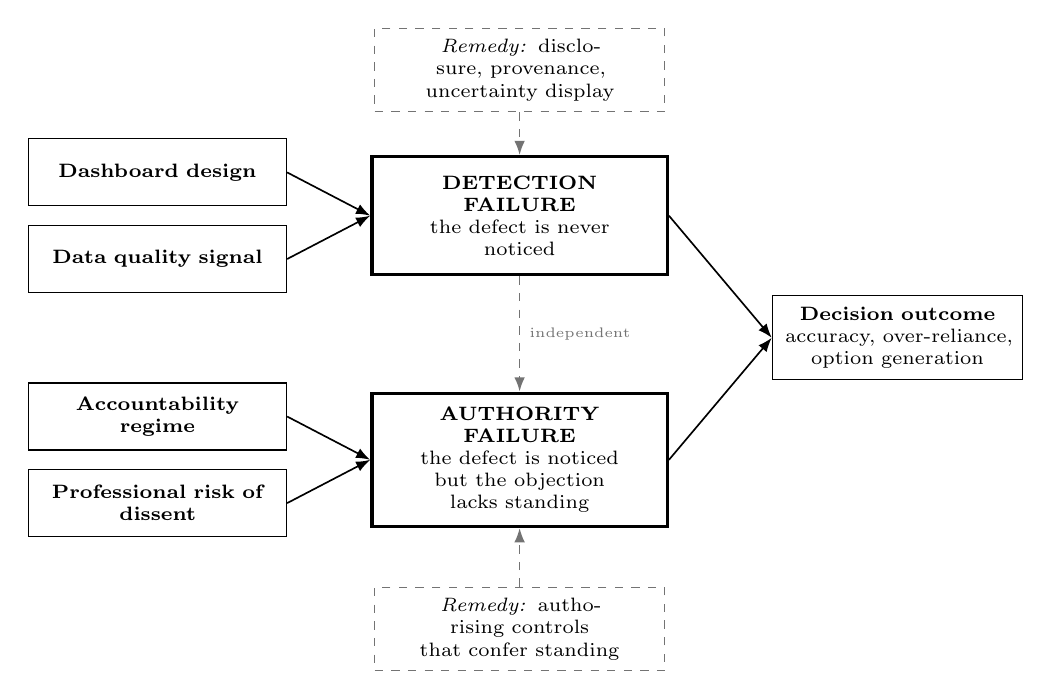
\begin{tikzpicture}[
  every node/.style={font=\scriptsize},
  ant/.style={draw=black,align=center,inner sep=4pt,text width=3.0cm,minimum height=0.85cm},
  mode/.style={draw=black,line width=1.2pt,align=center,inner sep=5pt,text width=3.4cm,minimum height=1.5cm},
  outc/.style={draw=black,align=center,inner sep=4pt,text width=2.9cm,minimum height=0.8cm},
  rem/.style={draw=black!55,dashed,align=center,inner sep=4pt,text width=3.4cm},
  ar/.style={-{Latex[length=1.8mm]},line width=0.6pt}]
\node[ant] (d1) at (0,2.4) {\textbf{Dashboard design}};
\node[ant] (d2) at (0,1.3) {\textbf{Data quality signal}};
\node[ant] (a1) at (0,-0.7) {\textbf{Accountability regime}};
\node[ant] (a2) at (0,-1.8) {\textbf{Professional risk of\\dissent}};
\node[mode] (m1) at (4.6,1.85) {\textbf{DETECTION FAILURE}\\\scriptsize the defect is never\\\scriptsize noticed};
\node[mode] (m2) at (4.6,-1.25) {\textbf{AUTHORITY FAILURE}\\\scriptsize the defect is noticed\\\scriptsize but the objection\\\scriptsize lacks standing};
\node[outc] (o) at (9.4,0.3) {\textbf{Decision outcome}\\\scriptsize accuracy, over-reliance,\\\scriptsize option generation};
\node[rem] (r1) at (4.6,3.7) {\emph{Remedy:} disclosure, provenance,\\uncertainty display};
\node[rem] (r2) at (4.6,-3.4) {\emph{Remedy:} authorising controls\\that confer standing};
\draw[ar] (d1.east) -- (m1.west); \draw[ar] (d2.east) -- (m1.west);
\draw[ar] (a1.east) -- (m2.west); \draw[ar] (a2.east) -- (m2.west);
\draw[ar] (m1.east) -- (o.west); \draw[ar] (m2.east) -- (o.west);
\draw[ar,black!55,dashed] (r1.south) -- (m1.north);
\draw[ar,black!55,dashed] (r2.north) -- (m2.south);
\draw[ar,black!55,dashed] (m1.south) -- node[right,font=\tiny]{independent} (m2.north);
\end{tikzpicture}
\caption{Revised conceptual framework, distinguishing detection failure from authority failure}
\label{fig:revised}
\end{figure}

The two modes possess different antecedents and different remedies, and they may occur independently of one
another. The documentary evidence indicates that authority failure was the operative mode in nine of the
twelve cases.

\section{What the documentary evidence cannot establish}

Intellectual honesty requires equal attention to the limits of this strand.

The sample is subject to severe survivorship bias. Only those failures which became public are observable
at all. Organisations in which a manager challenged a dashboard, was listened to, and quietly averted a
problem generate no inquiry report and appear nowhere in the dataset. Nothing at section 4.2 may therefore
be read as evidence regarding the \emph{frequency} of dashboard deference. The strand establishes the
anatomy of failure and not its base rate. This is precisely the limitation which the experimental strand is
designed to address, since a randomised vignette design does observe those cases in which challenge occurs.

Further, the cases are heterogeneous in ways which resist tidy comparison. A national air traffic
control system, a welfare debt raising algorithm and a transaction reporting pipeline differ in
their time constants, regulatory environment and proximity to the individual manager. The coding
frame imposes a common structure upon them, and the reader ought to retain some scepticism
regarding how much that structure genuinely reveals. This is the familiar trade-off in small-$n$
comparative work as between depth and comparability (Eisenhardt, 1989; Yin, 2018).

Finally, coding a construct such as legitimacy asymmetry necessarily involves interpretation. The double
coding procedure and the reliability statistic described at section 3.5.2 mitigate this difficulty but
cannot eliminate it, and the judgement remains a judgement.

\section{Implications for the remaining strands}

The documentary findings sharpen three expectations. Firstly, if authority rather than detection is the
binding constraint, then the manipulation of accountability framing at H2 should produce a larger effect
than the manipulation of data quality signal visibility at H1. This is a prediction which was not at all
obvious before the strand was analysed and which is now testable. Secondly, the interview protocol has been
revised so as to probe the detection versus authority distinction directly, by asking participants what
happened \emph{after} they last disagreed with a dashboard. Thirdly, the governance framework at section
6.2 should address authorising controls and not merely detective ones.

\blankbox{awaiting Strands 1 and 3}{%
This section will be completed with the theoretical, methodological and practical implications of the
integrated findings, and with an explicit account of any divergence between what the experiment shows, what
the interviews explain and what the documentary record contains.}

%=====================================================================
\chapt{6}{Conclusion}
%=====================================================================

\section{Provisional answers to the research questions}

On the evidence which is available at this stage, only the contextual component of RQ1 and a part of RQ2
can be addressed. The conditional and explanatory components await Strands 1 and 3.

As regards \textbf{RQ1}, the documentary record indicates that the decision conditions which are associated
with the gravest outcomes are the joint presence of a silent defect, an auditable accountability regime and
a control architecture which detects without authorising.

As regards \textbf{RQ2}, the record indicates that prioritisation of the system output persisted not
because contrary information was unavailable, but rather because the objection carried less institutional
weight than the output which it contradicted.

\section{Towards a governance framework}

The distinction between detection failure and authority failure yields a framework possessing two limbs
rather than one. Table~\ref{tab:gov} sets out its provisional form. It will be finalised once the remaining
strands have reported.

\begin{table}[H]
\centering\footnotesize
\caption{Provisional governance framework for preserving human challenge}
\label{tab:gov}
\begin{tabularx}{\textwidth}{@{}p{2.6cm} p{3.5cm} X@{}}
\toprule
\textbf{Failure mode} & \textbf{Control type} & \textbf{Practical measures indicated by the evidence} \\
\midrule
Detection failure & \emph{Detective controls}, which make the defect perceptible & Display data provenance
and freshness upon the face of the dashboard rather than in documentation; reconcile record counts as
between source and destination, the absence of which explains the Public Health England undercount; render
an absent feed as a visible gap rather than as a lower number \\
\addlinespace
Authority failure & \emph{Authorising controls}, which give standing to the person who disagrees & Provide
a recorded and escalable dissent route so that a contextual objection becomes an auditable artefact of
equal standing to the dashboard reading; require that the overriding of a documented challenge be itself
documented, with reasons; separate the person who may raise a concern from the person whose performance the
concern reflects upon \\
\addlinespace
Both & \emph{Design and review} & Treat any single source input to a consequential automated decision as a
control weakness; review whether reliance is being encouraged by framing decisions as auditable against the
system \\
\bottomrule
\end{tabularx}
\end{table}

\section{Contributions}

\textbf{\emph{Theoretical.}} The study distinguishes detection failure from authority failure and proposes
legitimacy asymmetry as the mechanism which links accountability regime to decision outcome. This extends
the automation bias literature, whose attentional account was developed in single operator settings and
does not readily accommodate an organisational hierarchy standing between the noticing and the deciding.

\textbf{\emph{Methodological.}} Two features are worth noting in this connection. Behaviour linked
interview sampling, in which participants are selected upon their observed experimental behaviour rather
than upon availability, makes a sequential design genuinely explanatory. Evidential grading of documentary
sources allows a reader to discount the weaker cases rather than requiring him or her to accept the sample
as uniform.

\textbf{\emph{Practical.}} The framework at section 6.2 indicates that governance investment which is
directed solely at better warnings addresses the failure mode which was \emph{not} operative in the
majority of the documented cases.

\section{Limitations}

The limitations of the design are set out at section 3.8 and those of the documentary strand at section
5.3, and they are not repeated here. Two overarching limitations should nonetheless be recorded. Firstly,
at the date of this draft two of the three strands remain incomplete, and consequently every conclusion
stated above is provisional and may be overturned. Secondly, the study examines a mechanism and not a
population. Even when it is complete it will support claims regarding how dashboard reliance operates
rather than claims regarding how widespread it is.

\section{Recommendations for further research}

Three directions follow from the present work. A field study within a single organisation, comparing
decision episodes before and after the introduction of a recorded dissent route, would test the authorising
control proposition directly. A replication in a generative artificial intelligence setting would establish
whether fluent system generated narrative strengthens legitimacy asymmetry beyond what a numeric dashboard
achieves. Finally, a study sampling upon \emph{averted} failures rather than upon realised ones, for
instance through near-miss registers, would address the survivorship bias which no design based upon public
failure documents can overcome.

\section{Concluding remark}

The documentary record of twelve organisational failures suggests that the risk posed by business
intelligence systems has been somewhat mischaracterised. The prevailing account holds that the danger lies
in managers failing to notice that a system is wrong. The evidence assembled here points elsewhere. In the
substantial majority of these cases somebody did notice, and said so, and the failure lay in what happened
next. The study therefore asks not whether dashboards ought to be used, for plainly they ought to be, but
rather how managers may remain decision makers within organisations in which dashboards have become the
most powerful voice in the room.

%=====================================================================
\newpage
\phantomsection\label{toc:refs}
\begin{center}{\large\bfseries References}\end{center}
\addtocontents{toc}{\protect\vspace{9pt}}
\addtocontents{toc}{\protect\noindent{\protect\bfseries References}\protect\dotfill\protect\pageref{toc:refs}\protect\par\protect\vspace{3pt}}
%=====================================================================
\vspace{10pt}

{\setstretch{1.25}
\setlength{\parskip}{7pt}
\newcommand{\rf}{\par\hangindent=1.2em\hangafter=1\noindent}

\rf Aguinis, H. and Bradley, K.J. (2014) `Best practice recommendations for designing and implementing experimental vignette methodology studies', \emph{Organizational Research Methods}, Vol. 17(4), pp. 351--371.

\rf Amabile, T.M. (1998) `How to kill creativity', \emph{Harvard Business Review}, Vol. 76(5), pp. 76--87.

\rf Anderson, N., Potočnik, K. and Zhou, J. (2014) `Innovation and creativity in organizations: a state-of-the-science review, prospective commentary, and guiding framework', \emph{Journal of Management}, Vol. 40(5), pp. 1297--1333.

\rf Arnott, D. and Pervan, G. (2005) `A critical analysis of decision support systems research', \emph{Journal of Information Technology}, Vol. 20(2), pp. 67--87.

\rf Atzmüller, C. and Steiner, P.M. (2010) `Experimental vignette studies in survey research', \emph{Methodology}, Vol. 6(3), pp. 128--138.

\rf Autoriteit Persoonsgegevens (2021) \emph{Tax Administration Fined for Discriminatory and Unlawful Data Processing}. The Hague: Dutch Data Protection Authority. Available at: https://www.autoriteitpersoonsgegevens.nl/en/current/tax-administration-fined-for-discriminatory-and-unlawful-data-processing (Accessed: 18 August 2026).

\rf Bach, B., Freeman, E., Abdul-Rahman, A., Turkay, C., Khan, S., Fan, Y. and Chen, M. (2023) `Dashboard design patterns', \emph{IEEE Transactions on Visualization and Computer Graphics}, Vol. 29(1), pp. 342--352.

\rf Bhaskar, R. (2008) \emph{A Realist Theory of Science}. Abingdon: Routledge.

\rf Bowen, G.A. (2009) `Document analysis as a qualitative research method', \emph{Qualitative Research Journal}, Vol. 9(2), pp. 27--40.

\rf Braun, V. and Clarke, V. (2006) `Using thematic analysis in psychology', \emph{Qualitative Research in Psychology}, Vol. 3(2), pp. 77--101.

\rf Bryman, A. (2016) \emph{Social Research Methods}. 5th edn. Oxford: Oxford University Press.

\rf Buçinca, Z., Malaya, M.B. and Gajos, K.Z. (2021) `To trust or to think: cognitive forcing functions can reduce overreliance on AI in AI-assisted decision-making', \emph{Proceedings of the ACM on Human-Computer Interaction}, Vol. 5(CSCW1), article 188.

\rf Burton, J.W., Stein, M.-K. and Jensen, T.B. (2020) `A systematic review of algorithm aversion in augmented decision making', \emph{Journal of Behavioral Decision Making}, Vol. 33(2), pp. 220--239.

\rf Chen, H., Chiang, R.H.L. and Storey, V.C. (2012) `Business intelligence and analytics: from big data to big impact', \emph{MIS Quarterly}, Vol. 36(4), pp. 1165--1188.

\rf Civil Aviation Authority (2024) \emph{CAP2993: Independent Review of NATS (En Route) Plc's Flight Planning System Failure on 28 August 2023. Final Report}. London: Civil Aviation Authority. Available at: https://www.caa.co.uk/CAP2993 (Accessed: 18 August 2026).

\rf Cleveland, W.S. and McGill, R. (1984) `Graphical perception: theory, experimentation, and application to the development of graphical methods', \emph{Journal of the American Statistical Association}, Vol. 79(387), pp. 531--554.

\rf Cohen, J. (1960) `A coefficient of agreement for nominal scales', \emph{Educational and Psychological Measurement}, Vol. 20(1), pp. 37--46.

\rf Cohen, J. (1988) \emph{Statistical Power Analysis for the Behavioral Sciences}. 2nd edn. Hillsdale, NJ: Lawrence Erlbaum Associates.

\rf Creswell, J.W. and Plano Clark, V.L. (2018) \emph{Designing and Conducting Mixed Methods Research}. 3rd edn. Thousand Oaks, CA: SAGE.

\rf Dietvorst, B.J., Simmons, J.P. and Massey, C. (2015) `Algorithm aversion: people erroneously avoid algorithms after seeing them err', \emph{Journal of Experimental Psychology: General}, Vol. 144(1), pp. 114--126.

\rf Doshi, A.R. and Hauser, O.P. (2024) `Generative AI enhances individual creativity but reduces the collective diversity of novel content', \emph{Science Advances}, Vol. 10(28), article eadn5290.

\rf Eisenhardt, K.M. (1989) `Building theories from case study research', \emph{Academy of Management Review}, Vol. 14(4), pp. 532--550.

\rf Elbashir, M.Z., Collier, P.A. and Davern, M.J. (2008) `Measuring the effects of business intelligence systems: the relationship between business process and organizational performance', \emph{International Journal of Accounting Information Systems}, Vol. 9(3), pp. 135--153.

\rf Espeland, W.N. and Sauder, M. (2007) `Rankings and reactivity: how public measures recreate social worlds', \emph{American Journal of Sociology}, Vol. 113(1), pp. 1--40.

\rf Field, A. (2018) \emph{Discovering Statistics Using IBM SPSS Statistics}. 5th edn. London: SAGE.

\rf Financial Conduct Authority (2019) \emph{Final Notice: Goldman Sachs International}. London: Financial Conduct Authority. Available at: https://www.fca.org.uk/publication/final-notices/goldman-sachs-international-2019.pdf (Accessed: 18 August 2026).

\rf Financial Conduct Authority (2022) \emph{Final Notice: TSB Bank plc}. London: Financial Conduct Authority. Available at: https://www.fca.org.uk/publication/final-notices/tsb-bank-plc-2022.pdf (Accessed: 18 August 2026).

\rf Franco-Santos, M. and Otley, D. (2018) `Reviewing and theorizing the unintended consequences of performance management systems', \emph{International Journal of Management Reviews}, Vol. 20(3), pp. 696--730.

\rf Goddard, K., Roudsari, A. and Wyatt, J.C. (2012) `Automation bias: a systematic review of frequency, effect mediators, and mitigators', \emph{Journal of the American Medical Informatics Association}, Vol. 19(1), pp. 121--127.

\rf Guest, G., Bunce, A. and Johnson, L. (2006) `How many interviews are enough? An experiment with data saturation and variability', \emph{Field Methods}, Vol. 18(1), pp. 59--82.

\rf Gunasekaran, A., Papadopoulos, T., Dubey, R., Wamba, S.F., Childe, S.J., Hazen, B. and Akter, S. (2017) `Big data and predictive analytics for supply chain and organizational performance', \emph{Journal of Business Research}, Vol. 70, pp. 308--317.

\rf Janssen, M., van der Voort, H. and Wahyudi, A. (2017) `Factors influencing big data decision-making quality', \emph{Journal of Business Research}, Vol. 70, pp. 338--345.

\rf Kache, F. and Seuring, S. (2017) `Challenges and opportunities of digital information at the intersection of big data analytics and supply chain management', \emph{International Journal of Operations \& Production Management}, Vol. 37(1), pp. 10--36.

\rf Kahneman, D. (2011) \emph{Thinking, Fast and Slow}. London: Penguin.

\rf Kellogg, K.C., Valentine, M.A. and Christin, A. (2020) `Algorithms at work: the new contested terrain of control', \emph{Academy of Management Annals}, Vol. 14(1), pp. 366--410.

\rf Krippendorff, K. (2018) \emph{Content Analysis: An Introduction to Its Methodology}. 4th edn. Thousand Oaks, CA: SAGE.

\rf Landis, J.R. and Koch, G.G. (1977) `The measurement of observer agreement for categorical data', \emph{Biometrics}, Vol. 33(1), pp. 159--174.

\rf Lebovitz, S., Lifshitz-Assaf, H. and Levina, N. (2022) `To engage or not to engage with AI for critical judgments: how professionals deal with opacity when using AI for medical diagnosis', \emph{Organization Science}, Vol. 33(1), pp. 126--148.

\rf Lincoln, Y.S. and Guba, E.G. (1985) \emph{Naturalistic Inquiry}. Beverly Hills, CA: SAGE.

\rf Logg, J.M., Minson, J.A. and Moore, D.A. (2019) `Algorithm appreciation: people prefer algorithmic to human judgment', \emph{Organizational Behavior and Human Decision Processes}, Vol. 151, pp. 90--103.

\rf Lyell, D. and Coiera, E. (2017) `Automation bias and verification complexity: a systematic review', \emph{Journal of the American Medical Informatics Association}, Vol. 24(2), pp. 423--431.

\rf Mahmud, H., Islam, A.K.M.N., Ahmed, S.I. and Smolander, K. (2022) `What influences algorithmic decision-making? A systematic literature review on algorithm aversion', \emph{Technological Forecasting and Social Change}, Vol. 175, article 121390.

\rf Market Research Society (2019) \emph{MRS Code of Conduct}. London: Market Research Society.

\rf Mikalef, P. and Gupta, M. (2021) `Artificial intelligence capability: conceptualization, measurement calibration, and empirical study on its impact on organizational creativity and firm performance', \emph{Information \& Management}, Vol. 58(3), article 103434.

\rf Mosier, K.L., Skitka, L.J., Heers, S. and Burdick, M. (1998) `Automation bias: decision making and performance in high-tech cockpits', \emph{The International Journal of Aviation Psychology}, Vol. 8(1), pp. 47--63.

\rf Nagle, T., Redman, T. and Sammon, D. (2020) `Assessing data quality: a managerial call to action', \emph{Business Horizons}, Vol. 63(3), pp. 325--337.

\rf Office for Statistics Regulation (2021) \emph{Ensuring Statistical Models Command Public Confidence: Learning Lessons from the Approach to Developing Models for Awarding Grades in the UK in 2020}. London: UK Statistics Authority. Available at: https://osr.statisticsauthority.gov.uk/publication/ensuring-statistical-models-command-public-confidence/ (Accessed: 18 August 2026).

\rf Office of the Comptroller of the Currency (2020) \emph{OCC Assesses \$400 Million Civil Money Penalty Against Citibank}. News release NR 2020-132. Washington, DC: Office of the Comptroller of the Currency. Available at: https://www.occ.gov/news-issuances/news-releases/2020/nr-occ-2020-132.html (Accessed: 18 August 2026).

\rf Parasuraman, R. and Manzey, D.H. (2010) `Complacency and bias in human use of automation: an attentional integration', \emph{Human Factors}, Vol. 52(3), pp. 381--410.

\rf Parasuraman, R. and Riley, V. (1997) `Humans and automation: use, misuse, disuse, abuse', \emph{Human Factors}, Vol. 39(2), pp. 230--253.

\rf Pauwels, K., Ambler, T., Clark, B.H., LaPointe, P., Reibstein, D., Skiera, B., Wierenga, B. and Wiesel, T. (2009) `Dashboards as a service: why, what, how, and what research is needed?', \emph{Journal of Service Research}, Vol. 12(2), pp. 175--189.

\rf Pipino, L.L., Lee, Y.W. and Wang, R.Y. (2002) `Data quality assessment', \emph{Communications of the ACM}, Vol. 45(4), pp. 211--218.

\rf Podsakoff, P.M., MacKenzie, S.B., Lee, J.-Y. and Podsakoff, N.P. (2003) `Common method biases in behavioral research: a critical review of the literature and recommended remedies', \emph{Journal of Applied Psychology}, Vol. 88(5), pp. 879--903.

\rf Post Office Horizon IT Inquiry (2025) \emph{Volume 1 of the Post Office Horizon IT Inquiry's Final Report}. London: Post Office Horizon IT Inquiry. Available at: https://www.postofficehorizoninquiry.org.uk (Accessed: 18 August 2026).

\rf Redman, T.C. (1998) `The impact of poor data quality on the typical enterprise', \emph{Communications of the ACM}, Vol. 41(2), pp. 79--82.

\rf Royal Commission into the Robodebt Scheme (2023) \emph{Report}. Canberra: Commonwealth of Australia. Available at: https://robodebt.royalcommission.gov.au/publications/report (Accessed: 18 August 2026).

\rf Runco, M.A. and Jaeger, G.J. (2012) `The standard definition of creativity', \emph{Creativity Research Journal}, Vol. 24(1), pp. 92--96.

\rf Sambasivan, N., Kapania, S., Highfill, H., Akrong, D., Paritosh, P. and Aroyo, L.M. (2021) `Everyone wants to do the model work, not the data work: data cascades in high-stakes AI', in \emph{Proceedings of the 2021 CHI Conference on Human Factors in Computing Systems}. New York: ACM, article 39.

\rf Sarikaya, A., Correll, M., Bartram, L., Tory, M. and Fisher, D. (2019) `What do we talk about when we talk about dashboards?', \emph{IEEE Transactions on Visualization and Computer Graphics}, Vol. 25(1), pp. 682--692.

\rf Saunders, M., Lewis, P. and Thornhill, A. (2019) \emph{Research Methods for Business Students}. 8th edn. Harlow: Pearson.

\rf Securities and Exchange Commission (2013) \emph{In the Matter of Knight Capital Americas LLC}. Administrative Proceeding, Release No. 34-70694. Washington, DC: Securities and Exchange Commission. Available at: https://www.sec.gov/files/litigation/admin/2013/34-70694.pdf (Accessed: 18 August 2026).

\rf Seddon, P.B., Constantinidis, D., Tamm, T. and Dod, H. (2017) `How does business analytics contribute to business value?', \emph{Information Systems Journal}, Vol. 27(3), pp. 237--269.

\rf Shollo, A. and Galliers, R.D. (2016) `Towards an understanding of the role of business intelligence systems in organisational knowing', \emph{Information Systems Journal}, Vol. 26(4), pp. 339--367.

\rf Shrestha, Y.R., Ben-Menahem, S.M. and von Krogh, G. (2019) `Organizational decision-making structures in the age of artificial intelligence', \emph{California Management Review}, Vol. 61(4), pp. 66--83.

\rf Simon, H.A. (1955) `A behavioral model of rational choice', \emph{Quarterly Journal of Economics}, Vol. 69(1), pp. 99--118.

\rf Skitka, L.J., Mosier, K.L. and Burdick, M. (1999) `Does automation bias decision-making?', \emph{International Journal of Human-Computer Studies}, Vol. 51(5), pp. 991--1006.

\rf Strong, D.M., Lee, Y.W. and Wang, R.Y. (1997) `Data quality in context', \emph{Communications of the ACM}, Vol. 40(5), pp. 103--110.

\rf Tashakkori, A. and Teddlie, C. (eds.) (2010) \emph{SAGE Handbook of Mixed Methods in Social \& Behavioral Research}. 2nd edn. Thousand Oaks, CA: SAGE.

\rf Trieu, V.-H. (2017) `Getting value from business intelligence systems: a review and research agenda', \emph{Decision Support Systems}, Vol. 93, pp. 111--124.

\rf Tufte, E.R. (2001) \emph{The Visual Display of Quantitative Information}. 2nd edn. Cheshire, CT: Graphics Press.

\rf US House Committee on Transportation and Infrastructure (2020) \emph{Final Committee Report: The Design, Development \& Certification of the Boeing 737 MAX}. Washington, DC: US House of Representatives.

\rf Vasconcelos, H., Jörke, M., Grunde-McLaughlin, M., Gerstenberg, T., Bernstein, M.S. and Krishna, R. (2023) `Explanations can reduce overreliance on AI systems during decision-making', \emph{Proceedings of the ACM on Human-Computer Interaction}, Vol. 7(CSCW1), article 129.

\rf Wamba, S.F., Gunasekaran, A., Akter, S., Ren, S.J., Dubey, R. and Childe, S.J. (2017) `Big data analytics and firm performance: effects of dynamic capabilities', \emph{Journal of Business Research}, Vol. 70, pp. 356--365.

\rf Wang, R.Y. and Strong, D.M. (1996) `Beyond accuracy: what data quality means to data consumers', \emph{Journal of Management Information Systems}, Vol. 12(4), pp. 5--33.

\rf Ware, C. (2013) \emph{Information Visualization: Perception for Design}. 3rd edn. Waltham, MA: Morgan Kaufmann.

\rf Woodman, R.W., Sawyer, J.E. and Griffin, R.W. (1993) `Toward a theory of organizational creativity', \emph{Academy of Management Review}, Vol. 18(2), pp. 293--321.

\rf Yigitbasioglu, O.M. and Velcu, O. (2012) `A review of dashboards in performance management: implications for design and research', \emph{International Journal of Accounting Information Systems}, Vol. 13(1), pp. 41--59.

\rf Yin, R.K. (2018) \emph{Case Study Research and Applications: Design and Methods}. 6th edn. Thousand Oaks, CA: SAGE.

\rf Zillow Group (2021) \emph{Third Quarter 2021 Shareholder Letter}. Seattle, WA: Zillow Group. Filed with the US Securities and Exchange Commission. Available at: https://www.sec.gov/Archives/edgar/data/1617640/000161764021000085/q32021991.htm (Accessed: 18 August 2026).
\par}

%=====================================================================
\newpage
\phantomsection\label{toc:apps}
\begin{center}{\large\bfseries Appendices}\end{center}
\addtocontents{toc}{\protect\vspace{9pt}}
\addtocontents{toc}{\protect\noindent{\protect\bfseries Appendices}\protect\dotfill\protect\pageref{toc:apps}\protect\par\protect\vspace{3pt}}
%=====================================================================
\setcounter{chapno}{0}
\setcounter{section}{0}
\renewcommand{\thetable}{\Alph{section}.\arabic{table}}
\renewcommand{\thefigure}{\Alph{section}.\arabic{figure}}
\newcommand{\appx}[1]{%
  \refstepcounter{section}\setcounter{table}{0}\setcounter{figure}{0}%
  \addcontentsline{toc}{subsection}{Appendix \Alph{section}. #1}%
  \vspace{8pt}\par\noindent{\normalsize\bfseries Appendix \Alph{section}.\hspace{0.7em}#1}\par
  \vspace{2pt}}

\appx{Literature Review Table}

\begin{longtable}{@{}p{2.4cm} p{2.5cm} p{2.0cm} p{2.1cm} p{2.5cm} p{2.6cm}@{}}
\caption{Ten key papers, with critical appraisal and use in this study}\\
\toprule
\footnotesize\textbf{Author (year)} & \footnotesize\textbf{Question addressed} &
\footnotesize\textbf{Theory} & \footnotesize\textbf{Method} & \footnotesize\textbf{Key finding} &
\footnotesize\textbf{Limitation and use here} \\
\midrule
\endfirsthead
\toprule
\footnotesize\textbf{Author (year)} & \footnotesize\textbf{Question addressed} &
\footnotesize\textbf{Theory} & \footnotesize\textbf{Method} & \footnotesize\textbf{Key finding} &
\footnotesize\textbf{Limitation and use here} \\
\midrule
\endhead
\bottomrule
\endfoot
\footnotesize Simon (1955) & How do people choose under cognitive limits? & Bounded rationality &
Theoretical & Decision makers satisfice rather than optimise & Pre-dates digital decision aids; explains
why an authoritative cue terminates search \\
\addlinespace
\footnotesize Parasuraman and Manzey (2010) & Why do operators over-trust automation? & Attentional
allocation & Integrative review & Reliance reduces attentional sampling of raw evidence & Aviation and
process control settings with formal escalation; supplies the detection mechanism only \\
\addlinespace
\footnotesize Dietvorst et al. (2015) & Do people abandon algorithms after error? & Algorithm
aversion & Laboratory experiments & Observing error causes disproportionate abandonment & Student samples,
generic forecasting, no accountability; supports H4b \\
\addlinespace
\footnotesize Logg et al. (2019) & Do people prefer algorithmic or human advice? & Advice taking &
Six experiments & General preference for algorithmic advice & Contradicts the aversion findings; motivates
the conditional framing of RQ1 \\
\addlinespace
\footnotesize Burton et al. (2020) & When does algorithm aversion occur? & Augmented decision making
& Systematic review & Reliance is condition dependent and not a stable trait & Synthesises heterogeneous
tasks; core justification for the scenario design \\
\addlinespace
\footnotesize Sarikaya et al. (2019) & What does dashboard design afford? & Visualisation design
space & Design space analysis & Dashboard types differ sharply in what users may notice & Descriptive
rather than behavioural; grounds the salience manipulation \\
\addlinespace
\footnotesize Wang and Strong (1996) & What does data quality mean to consumers? & Data quality dimensions &
Two stage survey & Quality is multidimensional and consumer defined & Built for assessment and not for
predicting behaviour; defines the data quality manipulation \\
\addlinespace
\footnotesize Nagle et al. (2020) & How well do firms measure data quality? & Managerial data quality
practice & Practitioner study & Organisations systematically under-measure quality & Reports extent of
under-measurement and not behavioural response; evidences the invisibility premise \\
\addlinespace
\footnotesize Espeland and Sauder (2007) & How do public measures change organisations? & Reactivity &
Qualitative field study & Measures reconstitute the reality they claim to describe & Single sector;
theoretical basis for legitimacy asymmetry and for H2 \\
\addlinespace
\footnotesize Lebovitz et al. (2022) & How do professionals handle opaque AI? & Knowledge work and
opacity & Comparative field study & Professionals disengage judgement where challenge is costly &
Healthcare only; directly informs the interview protocol \\
\end{longtable}

\newpage
\appx{Philosophical Positions Considered}

The philosophical argument is stated at section 3.1. Table~\ref{tab:phil} records the full comparison
of the positions considered and the basis for the position adopted.

\begin{table}[H]
\centering\footnotesize
\caption{Philosophical positions considered, and the basis for the position adopted}
\label{tab:phil}
\begin{tabularx}{\textwidth}{@{}p{2.6cm} X p{4.6cm}@{}}
\toprule
\textbf{Position} & \textbf{Implication for this study} & \textbf{Assessment} \\
\midrule
Positivism & Deference is an observable regularity to be measured and generalised. & Rejected. Captures
the experimental strand but cannot accommodate legitimacy, which is neither directly observable nor stable
across settings. \\
Interpretivism & Deference is meaning constructed by professionals in context. & Rejected as a sole
position. Captures RQ2 but forbids the controlled comparison which RQ1 requires. \\
Critical realism & Observable deference is generated by underlying mechanisms operating under particular
conditions. & \textbf{Adopted.} Licenses both measurement of the event and interpretation of the mechanism,
and makes conditionality the object of study rather than a nuisance. \\
Pragmatism & Methods are warranted by their capacity to answer the question rather than by paradigm
allegiance. & \textbf{Adopted as the practical orientation}, following established mixed methods guidance
(Creswell and Plano Clark, 2018; Tashakkori and Teddlie, 2010). \\
\bottomrule
\end{tabularx}
\end{table}

\newpage
\appx{Quality Criteria and Design Actions}

The quality criteria are summarised at section 3.6. Table~\ref{tab:quality} maps each criterion onto
the specific action taken in the corresponding strand.

\begin{table}[H]
\centering\footnotesize
\caption{Quality criteria and the corresponding design actions}
\label{tab:quality}
\begin{tabularx}{\textwidth}{@{}p{1.6cm} p{3.0cm} X@{}}
\toprule
\textbf{Strand} & \textbf{Criterion} & \textbf{Action taken} \\
\midrule
1 & Internal validity & Randomised and counterbalanced vignette allocation; within-subjects design;
manipulation checks \\
1 & Construct validity & Two independent coders for the creativity count; attention and comprehension
checks; pilot testing of cue salience \\
1 & External validity & Practising professionals rather than students; realistic dashboards; vignette
stakes acknowledged as lower than real ones \\
1 & Common method bias & Outcome is a behavioural choice rather than a self report; predictors are
manipulated rather than measured (Podsakoff et al., 2003) \\
2 & Documentary authenticity & Only independently verifiable primary documents admitted; evidential grading
applied and reported \\
2 & Coding reliability & Fixed extraction frame; thirty per cent double coding; Cohen's $\kappa$ reported \\
3 & Credibility & Behaviour linked sampling; member checking of summarised themes \\
3 & Dependability & Audit trail of coding decisions and analytic memos \\
3 & Transferability & Thick description of participant sector, role and context \\
3 & Reflexivity & The analytics training of the researcher creates a plausible bias towards reading
deference as error; coding therefore actively seeks accounts in which deference proved correct \\
\bottomrule
\end{tabularx}
\end{table}

\newpage
\appx{Reference Accessibility Register}

Every source cited has been checked for accessibility and has been recorded in a separate register
supplied alongside this document (\texttt{Sharma\_250559280\_Reference\_Register.xlsx}). The register records, in
respect of each source, the full Harvard citation; the source type; the DOI or stable URL; the verified
access status; the access route, namely open access or Newcastle University Library subscription; the
section in which the source is used; and a short statement of its relation to the argument.

\vspace{10pt}
\appx{Interview Guide}

\textbf{Preamble.} Purpose of the study; voluntary participation; anonymity and pseudonymisation; consent
to record; explicit instruction not to disclose confidential, client or commercially sensitive information;
right to pause, to skip or to withdraw.

\begin{enumerate}[leftmargin=*,itemsep=3pt,topsep=4pt]
\item Kindly tell me about the dashboards or reports which you use in a typical week. What is the first
thing that you look at?
\item Please walk me through a recent decision which started from a dashboard. What did you notice first?
What did you check?
\item Can you think of an occasion when a dashboard told you something which you did not believe? What did
you do? \textbf{And what happened after that?}
\item How do you know whether the numbers you are looking at are current and complete? What would make you
doubt them?
\item If a decision is questioned later, what evidence carries weight in your organisation? Is a data based
decision easier to defend than a judgement based one?
\item \emph{(Anonymised feedback on the participant's own experimental pattern.)} In one scenario the
dashboard signalled X whilst the local report suggested Y, and you chose\ldots\ What would drive your
choice in real life?
\item When you rely upon a dashboard, does it change the range of options which you consider? Which options
never make it onto the table?
\item What would need to be true, whether in the tool, the process or the culture, for people to push back
more often?
\item Is there anything important about this which I have not asked?
\end{enumerate}

\textbf{Closing.} Demographic items; debrief; contact details for follow-up or for withdrawal.

\vspace{10pt}
\appx{Documentary Source Index}

The following publication indices were searched systematically for Strand 2: Office of the Comptroller of
the Currency enforcement actions; Financial Conduct Authority final notices; Information Commissioner's
Office enforcement register; Autoriteit Persoonsgegevens enforcement decisions; United Kingdom statutory
public inquiry report libraries; Australian royal commission publications; National Audit Office value for
money reports; House of Commons select committee reports; United States Securities and Exchange Commission
administrative proceedings; Civil Aviation Authority CAP publications; and listed company annual report
restatement disclosures.

\vspace{10pt}
\appx{NVivo Literature Search Documentation}

\blankbox{screenshots to be captured and inserted before final submission}{%
The following will be captured from the NVivo project and inserted at this place: the keyword search
strategy and the Boolean strings used; the publication year distribution of the retrieved corpus; the word
frequency or concept map of the coded literature; and the coding structure showing the five argument steps
of Chapter 2.}

\vspace{10pt}
\appx{Survey Instrument}

\blankbox{instrument supplied as a separate file}{%
The full scenario based decision instrument, comprising the participant information sheet, the consent
items, the eight vignettes with their dashboard images, the outcome measures and the demographic items, is
supplied alongside this document as \texttt{Sharma\_250559280\_Survey\_Instrument.pdf}. It will be
reproduced in full at this appendix in the final submission.}

\end{document}
